%% Supplementary Information, compiled separately from main.tex so it can be uploaded as its own
%% file. Same class and figure path as the manuscript. Tables S2-S14 are generated from
%% results/tables by scripts/29_supplementary_tables.py (supp_tables.tex); S1 is written here.
\documentclass[pdflatex,sn-nature]{sn-jnl}

\usepackage{graphicx}
\usepackage{amsmath,amssymb,amsfonts}
\usepackage{booktabs}
\usepackage{longtable}
\usepackage{tabularx}
\usepackage{textcomp}
\usepackage{url}
\newcolumntype{L}{>{\raggedright\arraybackslash}X}

%% Cross-document references into the manuscript, so "Table 1" is never typed by hand. This reads
%% main.aux, so main.tex must be compiled first.
\usepackage{xr}
\externaldocument{main}

\graphicspath{{../../results/figures/}}
% Generated by scripts/18_manuscript_numbers.py. Do not edit by hand.
\newcommand{\nSourceRows}{161}  % T01
\newcommand{\nSourceKegg}{123}  % T01
\newcommand{\nZhuAcc}{259}  % T01
\newcommand{\nWuAcc}{301}  % T01
\newcommand{\nCaldanaMin}{14}  % T01
\newcommand{\nCaldanaMax}{18}  % T01
\newcommand{\nRefCompounds}{96}  % T02
\newcommand{\nRefRobust}{45}  % T02
\newcommand{\nRefSingle}{22}  % T02
\newcommand{\nRefNone}{28}  % T02
\newcommand{\nRefConflicting}{1}  % T02
\newcommand{\nRefUp}{24}  % T02
\newcommand{\nRefDown}{43}  % T02
\newcommand{\leuZhu}{4.92}  % T01
\newcommand{\leuWu}{4.74}  % T01
\newcommand{\leuCaldana}{2.40}  % T01
\newcommand{\ileZhu}{3.15}  % T01
\newcommand{\ileWu}{4.42}  % T01
\newcommand{\gluWu}{-0.50}  % T01
\newcommand{\gluWuFrac}{97}  % T01
\newcommand{\glnWu}{-0.02}  % T01
\newcommand{\glnWuFrac}{50}  % T01
\newcommand{\serZhu}{-0.29}  % T01
\newcommand{\serZhuFrac}{83}  % T01
\newcommand{\malZhu}{-1.19}  % T01
\newcommand{\oxgZhu}{-1.68}  % T01
\newcommand{\asnCaldana}{1.51}  % T01
\newcommand{\ratioLeuVal}{2.8}  % T02
\newcommand{\ratioLeuAsn}{2.7}  % T02
\newcommand{\nModelCompounds}{21}  % first study T06
\newcommand{\nComparable}{6}  % T03
\newcommand{\nScored}{12}  % T03
\newcommand{\nModelAgree}{5}  % T03
\newcommand{\nModelDisagree}{1}  % T03
\newcommand{\nModelUntested}{6}  % T03
\newcommand{\nModelNotComparable}{9}  % T03
\newcommand{\nNotPredicted}{59}  % T03
\newcommand{\nNotPredictedRobust}{41}  % T03
\newcommand{\nTests}{36}  % T08
\newcommand{\nMatch}{18}  % T08
\newcommand{\nLitMatch}{5}  % T08
\newcommand{\nDarkMatch}{13}  % T08
\newcommand{\nLitTests}{18}  % T08
\newcommand{\nSigLitPredicted}{0}  % T08
\newcommand{\pDinFiveTwoTwo}{= 0.0281}  % T08
\newcommand{\qDinFiveTwoTwo}{= 0.127}  % T08
\newcommand{\zDinFiveTwoTwo}{2.4}  % T08
\newcommand{\pDinLight}{= 0.089}  % T08
\newcommand{\qDinLight}{= 0.229}  % T08
\newcommand{\zDinLight}{1.7}  % T08
\newcommand{\pDinFourTwoSeven}{= 0.0318}  % T08
\newcommand{\qDinFourTwoSeven}{= 0.127}  % T08
\newcommand{\zDinFourTwoSeven}{2.2}  % T08
\newcommand{\pBcaaLight}{= 0.0397}  % T08
\newcommand{\qBcaaLight}{= 0.143}  % T08
\newcommand{\zBcaaLight}{2.0}  % T08
\newcommand{\pDinThirtyEight}{= 0.0015}  % T08
\newcommand{\qDinThirtyEight}{= 0.0108}  % T08
\newcommand{\zDinThirtyEight}{-3.4}  % T08
\newcommand{\pDinThreeTwoOne}{\le 10^{-4}}  % T08
\newcommand{\qDinThreeTwoOne}{= 0.0018}  % T08
\newcommand{\zDinThreeTwoOne}{-5.6}  % T08
\newcommand{\pDinDark}{= 4.00\times10^{-4}}  % T08
\newcommand{\qDinDark}{= 0.0048}  % T08
\newcommand{\zDinDark}{3.9}  % T08
\newcommand{\pBcaaThreeTwoOne}{\le 10^{-4}}  % T08
\newcommand{\qBcaaThreeTwoOne}{= 0.0018}  % T08
\newcommand{\zBcaaThreeTwoOne}{-6.9}  % T08
\newcommand{\pBcaaDark}{= 1.00\times10^{-3}}  % T08
\newcommand{\qBcaaDark}{= 0.009}  % T08
\newcommand{\zBcaaDark}{3.4}  % T08
\newcommand{\pSharedLight}{= 0.0019}  % T08
\newcommand{\qSharedLight}{= 0.0114}  % T08
\newcommand{\zSharedLight}{2.8}  % T08
\newcommand{\pDarkMetFiveTwoTwo}{= 0.0281}  % T08
\newcommand{\qDarkMetFiveTwoTwo}{= 0.127}  % T08
\newcommand{\zDarkMetFiveTwoTwo}{2.1}  % T08
\newcommand{\pDinFiveTwoTwoMW}{= 0.0026}  % T08
\newcommand{\pDinFiveTwoTwoRot}{= 0.0087}  % T08
\newcommand{\pDinFirstStudy}{= 0.0026}  % first study T07
\newcommand{\nSetDin}{5}  % prereg/gene_sets.tsv
\newcommand{\nSetBcaa}{53}  % prereg/gene_sets.tsv
\newcommand{\nSetWuControl}{301}  % prereg/gene_sets.tsv
\newcommand{\nSetWuStress}{491}  % prereg/gene_sets.tsv
\newcommand{\nSetWuShared}{1{,}954}  % prereg/gene_sets.tsv
\newcommand{\nSetWuDarkMet}{540}  % prereg/gene_sets.tsv
\newcommand{\nPathOne}{6}  % T07
\newcommand{\nHubOne}{7}  % T07
\newcommand{\nHubTestedOne}{15}  % T07
\newcommand{\nPathA}{6}  % T07
\newcommand{\nHubA}{11}  % T07
\newcommand{\nHubTestedA}{32}  % T07
\newcommand{\nPathB}{24}  % T07
\newcommand{\nHubB}{17}  % T07
\newcommand{\nHubTestedB}{32}  % T07
\newcommand{\nPathC}{10}  % T07
\newcommand{\nHubC}{5}  % T07
\newcommand{\nHubTestedC}{32}  % T07
\newcommand{\rhoOneA}{0.95}  % T04
\newcommand{\rhoBC}{0.51}  % T04
\newcommand{\nPathTotal}{232}  % T04
\newcommand{\rankGlyOne}{214}  % T04
\newcommand{\rankGlyA}{193}  % T04
\newcommand{\pPhotoC}{= 1.03\times10^{-12}}  % T04
\newcommand{\qPhotoB}{= 0.131}  % T04
\newcommand{\pBcaaDegC}{= 0.00506}  % T04
\newcommand{\pBcaaDegB}{= 0.0854}  % T04
\newcommand{\pErA}{= 8.65\times10^{-9}}  % T04
\newcommand{\hubLightFDR}{0.044}  % T05
\newcommand{\nSharedHubSteps}{16}  % T07
\newcommand{\nLayer}{96}  % data/paintomics_upload/metabolomics_key.tsv
\newcommand{\nLayerRelevant}{45}  % data/paintomics_upload/metabolomics_key.tsv
\newcommand{\nDELight}{7{,}790}  % data/osdr/contrast_OSD-678-light
\newcommand{\nDEDark}{2{,}112}  % data/osdr/contrast_OSD-678-dark
\newcommand{\ratioDE}{3.7}  % data/osdr
\newcommand{\nPanel}{29}  % T10
\newcommand{\nPanelGroups}{19}  % data/reference/metabolights_group_sds.tsv
\newcommand{\nPanelStudies}{6}  % data/reference/metabolights_group_sds.tsv
\newcommand{\sdMin}{0.31}  % T10
\newcommand{\sdMax}{1.21}  % T10
\newcommand{\nQThousandMin}{92}  % T10
\newcommand{\nQThousandMax}{1{,}342}  % T10
\newcommand{\nQSixtyMin}{1{,}293}  % T10
\newcommand{\detectMin}{0.56}  % T10
\newcommand{\detectMinFold}{1.48}  % T10
\newcommand{\nTwoFoldMax}{24}  % T10
\newcommand{\qSixtyLogTwo}{0.035}  % first study T13


\renewcommand{\thefigure}{S\arabic{figure}}
\renewcommand{\thetable}{S\arabic{table}}

\begin{document}

\title[Supplementary information]{Supplementary information for: Natural variation in
\textit{Arabidopsis} darkness metabolism tests a carbon starvation model of spaceflight
transcriptomes}

%% AUTHORSHIP --- mirrors main.tex.
\author*[1,2]{\fnm{Richard} \sur{Barker}}\email{dr.richard.barker@gmail.com}
\affil[1]{\orgname{Department of Agricultural and Biological Engineering, Purdue University},
  \city{West Lafayette, IN}, \country{USA}}
\affil[2]{\orgname{The Collaborative Science Environment, PBC}, \country{USA}}

\maketitle

Everything here except Table~S1 was added in revision, in answer to a reviewer, and is post hoc:
the analysis plan is in \texttt{prereg/revision1/} (commit 90ff4b8; hypoxia-signature addendum
8d6a9ae), committed before these analyses ran but after the pre-registered results were known. The
pre-registered results (T02, T08, T12 and the T03 verdicts) are unchanged. Each table is generated
from the named results table in the repository.

\section*{Supplementary figures}

\begin{figure}[htbp]\centering
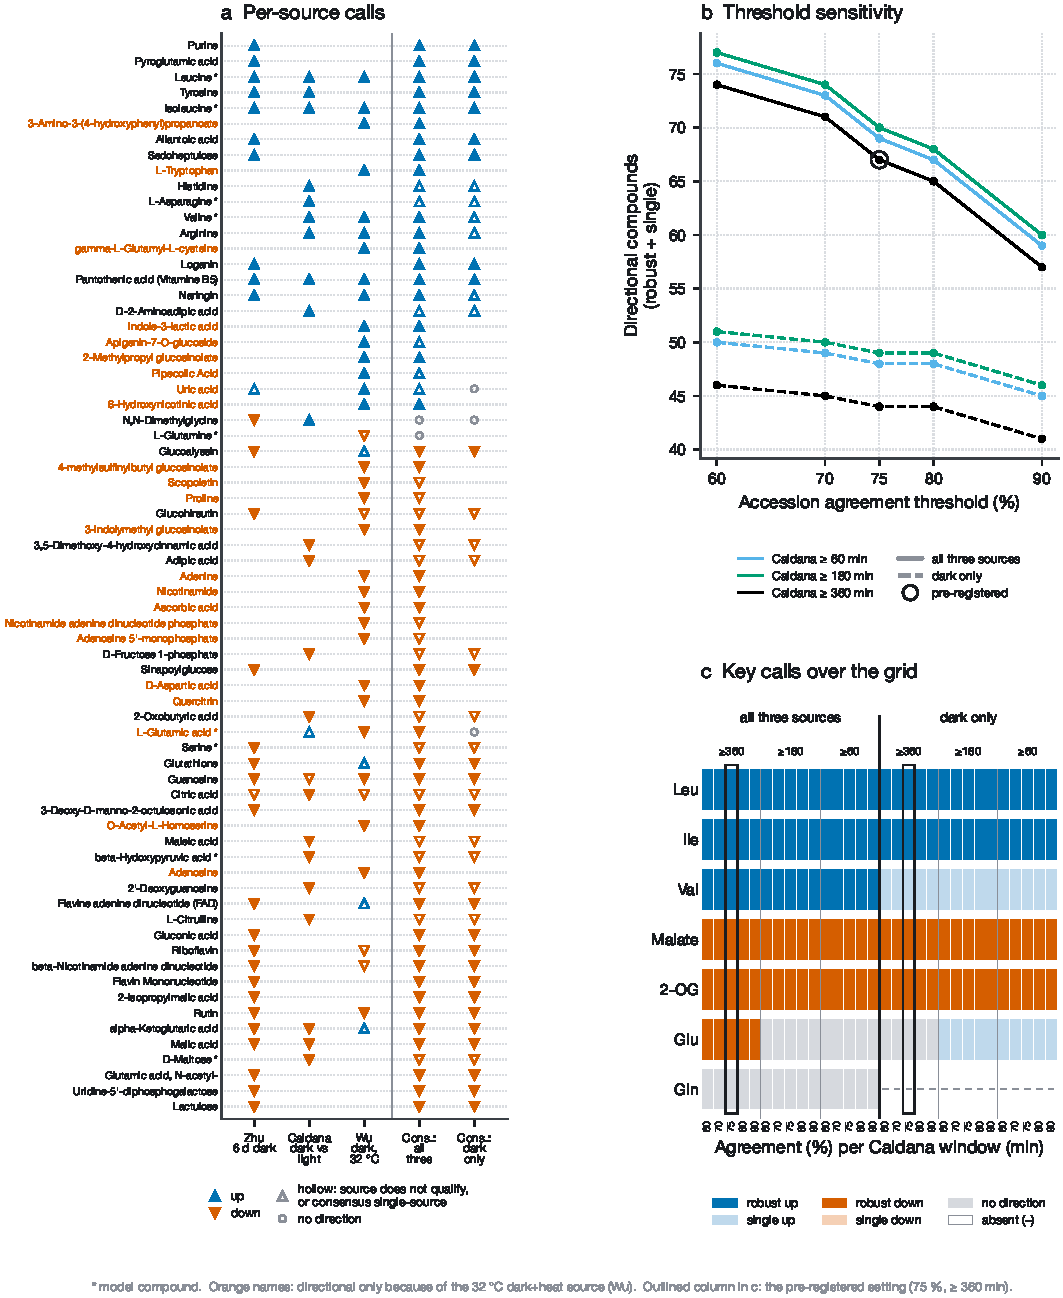
\includegraphics[width=\textwidth]{figS1_reference_strata.pdf}
\caption{\textbf{The darkness reference by source and stratum, and its threshold sensitivity.}
\textbf{a}, Per-source calls for every compound with a directional or conflicting consensus, or in
the model: filled symbols, the source qualifies (or the consensus is robust); hollow, it does not
(or the consensus rests on one source). Orange names are directional only because of the
32\,\textdegree C dark+heat source (Wu). \textbf{b}, Directional compounds over accession agreement
and Caldana window, for all three sources (solid) and darkness only (dashed). \textbf{c}, The key
calls over the same grid; the outlined columns are the pre-registered setting.}
\label{fig:s1}
\end{figure}

\begin{figure}[htbp]\centering
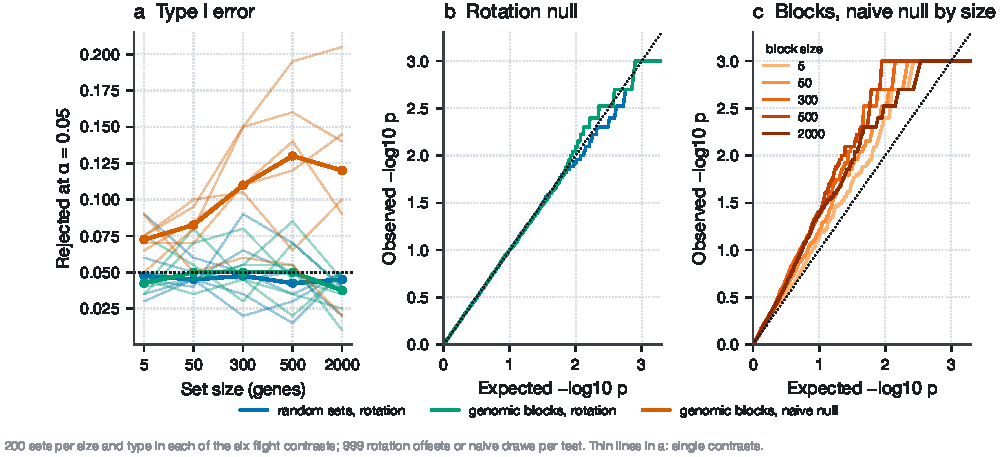
\includegraphics[width=\textwidth]{figS2_rotation_calibration.pdf}
\caption{\textbf{Calibration of the genomic-rotation null.} \textbf{a}, Share of 200 random gene
sets or contiguous genomic blocks rejected at $\alpha=0.05$, by set size; thin lines single flight
contrasts, thick lines their median. \textbf{b}, Quantile--quantile plot of rotation $p$-values,
pooled over contrasts and sizes. \textbf{c}, Genomic blocks against a naive random-gene null, by
block size: the inflation that gene clustering causes and the rotation null removes.}
\label{fig:s2}
\end{figure}

\begin{figure}[htbp]\centering
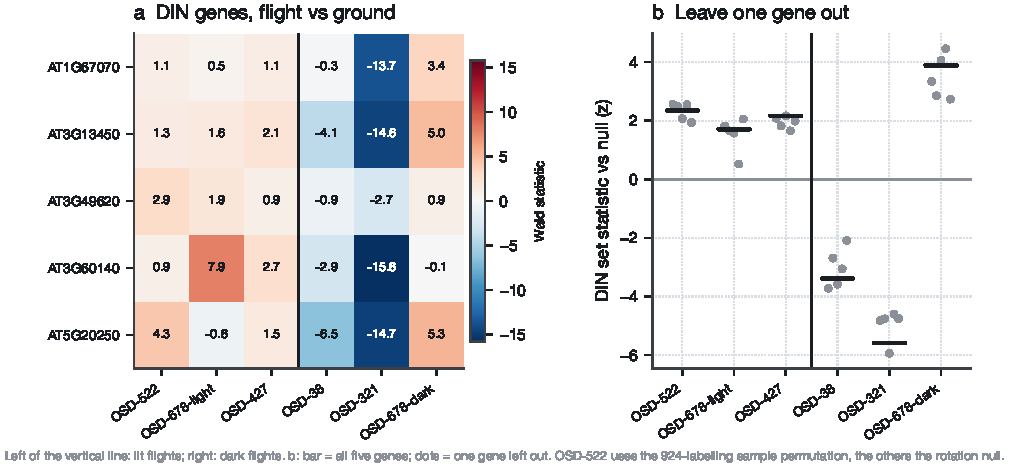
\includegraphics[width=\textwidth]{figS3_din_genes.pdf}
\caption{\textbf{The five DIN genes.} \textbf{a}, Wald statistic of each gene in each flight
contrast. \textbf{b}, The DIN set statistic against its null ($z$) with all five genes (bar) and
with each left out (dots).}
\label{fig:s3}
\end{figure}

\clearpage
\section*{Supplementary tables}

\begingroup\scriptsize
\begin{longtable}{@{}>{\raggedright\arraybackslash}p{2.2cm}>{\raggedright\arraybackslash}p{1.9cm}>{\raggedright\arraybackslash}p{5.2cm}>{\raggedright\arraybackslash}p{4.1cm}@{}}
\caption{\textbf{Where each entry of Table~\ref{tab:sources} and of the hardware and hypoxia
designs is stated.} Values as given by the source, condensed; ``not stated'' after searching the
full text or deposit. Wu et al.\ is read in its accepted manuscript (Wageningen University
repository, \url{https://edepot.wur.nl/426556}; line numbers are the manuscript's).}\label{tab:s1}\\
\toprule
Source & Field & Value & Where stated\\
\midrule
\endfirsthead
\toprule
Source & Field & Value & Where stated\\
\midrule
\endhead
\bottomrule
\endfoot
Zhu 2024 \citep{zhu2024} & Material & Leaf, 50\,mg ground; one plant per accession per timepoint & Methods, LC-MS analysis; Plant material and sample preparation\\
 & Age, growth & 35\,d after germination; short days in a greenhouse; photoperiod hours, light and temperature not stated & Plant material and sample preparation\\
 & Seasons & Autumn 2018 and spring 2019, two biological replicates & Plant material and sample preparation\\
 & Darkness & 0 and 6\,d; temperature in darkness not stated & Abstract; whole text searched\\
 & Sampling & Within 30\,min at 10:00 (GMT+2) & Plant material and sample preparation\\
 & Platform & Acquity UPLC with Exactive Orbitrap; negative mode, $m/z$ 100--1500 & LC-MS analysis\\
 & Values & BLUPs (lme4) over the two seasons; batches standardised to quality controls & Technical Validation; Plant material\\
 & Accessions & 259 & Plant material and sample preparation\\
Zhu 2022 \citep{zhu2022} & Growth & Short days, 8\,h light, 250\,$\mu$E\,m$^{-2}$\,s$^{-1}$, 20/16\,\textdegree C, humidity 60/75\,\% & Materials and methods, Plant materials and growth conditions\\
 & Sampling & At each harvest, within 30\,min at 10:00 (GMT+2) & Same\\
Wu 2018 \citep{wu2018} & Control & 16\,h light, 150\,$\mu$E\,m$^{-2}$\,s$^{-1}$, 20/16\,\textdegree C, humidity 60/75\,\% & Lines 510--512\\
 & Stress & Darkness, 32\,\textdegree C, humidity 75\,\%, continuous 1{,}280\,min, matching Caldana et al.'s stress & Lines 512--515\\
 & Age, harvest & Control harvested at 42\,d after germination, from 4\,h into the light period; stress plants after 1{,}280\,min & Lines 515--518\\
 & Material & About 100\,mg rosettes; three plants pooled per biological replicate & Lines 518--520, 548--550\\
 & Platform & Acquity UPLC with Exactive; positive and negative modes; day- and sample-median normalisation & Lines 558--570, 594--595\\
 & Filter & Traits present in at least 50\,\% of accessions & Lines 621--622\\
 & Accessions & 309 (314 less five with poor germination) & Lines 604--606\\
 & Time course & Material of Caldana et al.\ 2011, Col-0, re-profiled by LC--MS; conditions 21-D and 21-L (21\,\textdegree C, 150\,$\mu$E) among eight & Lines 176--186, 475--484\\
 & Column labels & Supplementary Table 7 labels conditions 4/20/30 (text: 4/21/32\,\textdegree C); the label key is not stated & Supplementary Table 7; text and Supplementary Information searched\\
Caldana 2011 \citep{caldana2011} & Conditions & Grown at 21\,\textdegree C, 150\,$\mu$E; kept there or moved to seven environments including 21\,\textdegree C darkness; 0 and 22 time points & Abstract (full text not accessible to us)\\
E-MTAB-375 \citep{emtab375} & Material & Columbia-0 (stock CS906), wild type, rosette leaf & Sample and data relationship file\\
OSD-38 \citep{osd38} & Comparator & 22 plates in sealed PDFUs in BRIC canisters at Kennedy Space Center; 22 plates in foil inside opaque, air-tight plastic containers at Ohio University; 4\,d cold, then 76\,h growth; continuous dark & OSDR growth protocol\\
 & Fixation & RNAlater, 12\,h, then $-80$\,\textdegree C, both arms & OSDR sample collection protocol\\
OSD-136 \citep{osd136,zhou2017} & Design & Wassilewskija roots, 5\,d old; 24\,h at 97\,kPa, 50\,kPa (O$_2$ 10\,kPa) or 50\,kPa with O$_2$ restored to 21\,kPa; three replicates & OSDR treatment protocol; Zhou et al., Abstract, Methods, Table 1\\
GSE14502 \citep{gse14502,mustroph2009} & Design & 7-d Col-0 seedlings (p35S:HF-RPL18), vertical MS plates, 23\,\textdegree C; 2\,h argon from the end of the light period; roots and shoots; total mRNA from the 35S line; ATH1 arrays, RMA & GEO sample records; Mustroph et al., Materials and Methods\\
\end{longtable}
\endgroup

% Generated by scripts/29_supplementary_tables.py from results/tables. Do not edit by hand.

\begingroup\tiny\setlength{\tabcolsep}{3pt}
\begin{longtable}{@{}llrrrlll@{}}
\caption{\textbf{Reference consensus by stratum (T14).} Per source: effect (log$_2$; * the source qualifies) and support (Zhu, Wu: share of accessions moving with the median, accessions in brackets; Caldana: Welch $p$, values in brackets). Consensus with all three sources (= T02) and with darkness only (Zhu, Caldana); ``dark+heat only'': directional only because of Wu's 32\,\textdegree C stress.}\label{tab:s2}\\
\toprule
Compound & KEGG & Zhu & Caldana & Wu (32\,\textdegree C) & All three & Dark only & Heat only \\
\midrule
\endfirsthead
\multicolumn{8}{l}{\textit{(continued)}}\\
\toprule
Compound & KEGG & Zhu & Caldana & Wu (32\,\textdegree C) & All three & Dark only & Heat only \\
\midrule
\endhead
\bottomrule
\endfoot
N,N-Dimethylglycine & C01026 & $-0.59$* / 100\,\% (259) & 0.93* / $1.6\times10^{-4}$ (18) & -- & confl. & confl. &  \\
L-Glutamine & C00064 & -- & -- & $-0.02$ / 50\,\% (301) & none & -- &  \\
Methionine & C00073 & -- & -- & 0.12 / 59\,\% (301) & none & -- &  \\
Choline & C00114 & -- & 0.01 / 0.946 (18) & -- & none & none &  \\
5'-Deoxy-5'-(methylthio)adenos & C00170 & -- & $-0.05$ / 0.580 (18) & -- & none & none &  \\
cis-Aconitic acid & C00417 & -- & -- & 0.14 / 57\,\% (301) & none & -- &  \\
Cytidine & C00475 & -- & $-0.09$ / 0.611 (18) & -- & none & none &  \\
5-Hydroxy-L-tryptophan & C00643 & -- & $-0.09$ / 0.381 (17) & -- & none & none &  \\
p-Coumaric acid & C00811 & -- & $-0.14$ / 0.450 (18) & -- & none & none &  \\
Saccharic acid & C00818 & $-0.10$ / 68\,\% (259) & -- & -- & none & none &  \\
4-Guanidinobutyric acid & C01035 & -- & 0.00 / 0.996 (18) & -- & none & none &  \\
Allantoin & C01551 & -- & 0.46 / 0.146 (18) & -- & none & none &  \\
Maltotriose & C01835 & -- & $-0.33$ / 0.273 (18) & -- & none & none &  \\
Benzyl glucosinolate & C02153 & -- & -- & 0.36 / 73\,\% (300) & none & -- &  \\
alpha-L-Fucose 1-phosphate & C02985 & -- & $-0.02$ / 0.922 (18) & -- & none & none &  \\
5-O-(Indol-3-ylacetyl-myo-inos & C04695 & -- & -- & $-0.57$ / 75\,\% (295) & none & -- &  \\
Allothreonine & C05519 & -- & $-0.36$ / 0.068 (18) & -- & none & none &  \\
N-Acetyl-D-phenylalanine & C05620 & -- & -- & $-0.22$ / 65\,\% (301) & none & -- &  \\
Nicotinate D-ribonucleoside & C05841 & -- & -- & $-0.09$ / 58\,\% (285) & none & -- &  \\
Hydroxymethylphosphonic acid & C06455 & -- & 0.06 / 0.664 (14) & -- & none & none &  \\
5-methylthiopentylglucosinolat & C08401 & -- & -- & 0.51 / 63\,\% (298) & none & -- &  \\
4-pentenylglucosinolate & C08403 & -- & -- & 0.16 / 53\,\% (192) & none & -- &  \\
4-methylthiobutyl glucosinolat & C08409 & -- & -- & 0.01 / 50\,\% (264) & none & -- &  \\
3-methylsulfinylpropyl-glucosi & C08411 & -- & -- & $-0.96$ / 73\,\% (199) & none & -- &  \\
3-methylthiopropyl-glucosinola & C08412 & -- & -- & $-0.21$ / 57\,\% (269) & none & -- &  \\
3-butenylglucosinolate & C08415 & -- & -- & $-0.04$ / 51\,\% (301) & none & -- &  \\
2-Picolinic acid & C10164 & -- & -- & 0.22 / 72\,\% (301) & none & -- &  \\
7-methylthioheptyl glucosinola & C17252 & -- & -- & 0.25 / 63\,\% (270) & none & -- &  \\
8-Methylthiooctyl glucosinolat & C17254 & -- & -- & 0.01 / 51\,\% (301) & none & -- &  \\
Purine & C15587 & 5.11* / 100\,\% (259) & -- & -- & robust $\uparrow$ & robust $\uparrow$ &  \\
Pyroglutamic acid & C01879 & 1.43* / 100\,\% (259) & -- & -- & robust $\uparrow$ & robust $\uparrow$ &  \\
Leucine & C00123 & 4.92* / 100\,\% (259) & 2.40* / $2.9\times10^{-8}$ (18) & 4.74* / 100\,\% (301) & robust $\uparrow$ & robust $\uparrow$ &  \\
Tyrosine & C00082 & 5.06* / 100\,\% (259) & 2.36* / $1.8\times10^{-6}$ (18) & -- & robust $\uparrow$ & robust $\uparrow$ &  \\
Isoleucine & C00407 & 3.15* / 100\,\% (259) & 2.17* / $2.7\times10^{-7}$ (18) & 4.42* / 100\,\% (301) & robust $\uparrow$ & robust $\uparrow$ &  \\
3-Amino-3-(4-hydroxyphenyl)pro & C04368 & -- & -- & 5.05* / 100\,\% (301) & robust $\uparrow$ & -- & yes \\
Allantoic acid & C00499 & 4.01* / 100\,\% (259) & -- & -- & robust $\uparrow$ & robust $\uparrow$ &  \\
Sedoheptulose & C02076 & 1.46* / 100\,\% (259) & -- & -- & robust $\uparrow$ & robust $\uparrow$ &  \\
L-Tryptophan & C00078 & -- & -- & 5.41* / 100\,\% (301) & robust $\uparrow$ & -- & yes \\
Valine & C00183 & -- & 0.90* / $4.3\times10^{-5}$ (18) & 2.49* / 100\,\% (301) & robust $\uparrow$ & single $\uparrow$ &  \\
Arginine & C00062 & -- & 2.58* / $1.8\times10^{-6}$ (18) & 2.34* / 100\,\% (301) & robust $\uparrow$ & single $\uparrow$ &  \\
gamma-L-Glutamyl-L-cysteine & C00669 & -- & -- & 2.39* / 100\,\% (301) & robust $\uparrow$ & -- & yes \\
Loganin & C01433 & 2.28* / 100\,\% (259) & -- & -- & robust $\uparrow$ & robust $\uparrow$ &  \\
Pantothenic acid (Vitamine B5) & C00864 & 1.26* / 100\,\% (259) & 0.25* / 0.019 (18) & 2.02* / 100\,\% (301) & robust $\uparrow$ & robust $\uparrow$ &  \\
Naringin & C09789 & 1.42* / 88\,\% (259) & -- & 0.36* / 81\,\% (298) & robust $\uparrow$ & single $\uparrow$ &  \\
Indole-3-lactic acid & C02043 & -- & -- & 1.00* / 94\,\% (301) & robust $\uparrow$ & -- & yes \\
2-Methylpropyl glucosinolate & C17256 & -- & -- & 1.26* / 93\,\% (284) & robust $\uparrow$ & -- & yes \\
6-Hydroxynicotinic acid & C01020 & -- & -- & 0.50* / 92\,\% (293) & robust $\uparrow$ & -- & yes \\
Glucoalyssin & C08400 & $-0.71$* / 96\,\% (259) & -- & 0.14 / 54\,\% (301) & robust $\downarrow$ & robust $\downarrow$ &  \\
4-methylsulfinylbutyl glucosin & C08419 & -- & -- & $-1.19$* / 96\,\% (199) & robust $\downarrow$ & -- & yes \\
3-indolymethyl glucosinolate & C05837 & -- & -- & $-0.51$* / 90\,\% (301) & robust $\downarrow$ & -- & yes \\
Adenine & C00147 & -- & -- & $-0.90$* / 93\,\% (301) & robust $\downarrow$ & -- & yes \\
Nicotinamide & C00153 & -- & -- & $-1.32$* / 92\,\% (301) & robust $\downarrow$ & -- & yes \\
Ascorbic acid & C00072 & -- & -- & $-1.61$* / 92\,\% (274) & robust $\downarrow$ & -- & yes \\
Sinapoylglucose & C01175 & $-0.73$* / 96\,\% (259) & -- & -- & robust $\downarrow$ & robust $\downarrow$ &  \\
D-Aspartic acid & C00049 & -- & -- & $-0.43$* / 92\,\% (301) & robust $\downarrow$ & -- & yes \\
Quercitrin & C01750 & -- & -- & $-1.97$* / 99\,\% (298) & robust $\downarrow$ & -- & yes \\
L-Glutamic acid & C00025 & -- & 0.08 / 0.337 (18) & $-0.51$* / 97\,\% (301) & robust $\downarrow$ & none & yes \\
Glutathione & C00051 & $-0.47$* / 98\,\% (259) & -- & 0.04 / 54\,\% (301) & robust $\downarrow$ & robust $\downarrow$ &  \\
Guanosine & C00387 & $-1.06$* / 99\,\% (259) & $-0.36$ / 0.062 (18) & $-0.93$* / 90\,\% (301) & robust $\downarrow$ & robust $\downarrow$ &  \\
3-Deoxy-D-manno-2-octulosonic  & C01187 & $-0.51$* / 100\,\% (259) & -- & -- & robust $\downarrow$ & robust $\downarrow$ &  \\
O-Acetyl-L-Homoserine & C01077 & -- & -- & $-1.45$* / 100\,\% (301) & robust $\downarrow$ & -- & yes \\
Adenosine & C00212 & -- & -- & $-1.32$* / 97\,\% (301) & robust $\downarrow$ & -- & yes \\
Flavine adenine dinucleotide ( & C00016 & $-0.80$* / 100\,\% (259) & -- & 0.28 / 69\,\% (300) & robust $\downarrow$ & robust $\downarrow$ &  \\
Gluconic acid & C00257 & $-0.38$* / 100\,\% (259) & -- & -- & robust $\downarrow$ & robust $\downarrow$ &  \\
Riboflavin & C00255 & $-1.11$* / 100\,\% (259) & -- & $-0.16$ / 65\,\% (301) & robust $\downarrow$ & robust $\downarrow$ &  \\
beta-Nicotinamide adenine dinu & C00003 & $-0.61$* / 100\,\% (259) & -- & $-0.00$ / 50\,\% (301) & robust $\downarrow$ & robust $\downarrow$ &  \\
Flavin Mononucleotide & C00061 & $-0.56$* / 100\,\% (259) & -- & -- & robust $\downarrow$ & robust $\downarrow$ &  \\
2-Isopropylmalic acid & C02504 & $-0.73$* / 98\,\% (259) & -- & -- & robust $\downarrow$ & robust $\downarrow$ &  \\
Rutin & C05625 & $-0.99$* / 99\,\% (259) & -- & $-0.63$* / 81\,\% (301) & robust $\downarrow$ & robust $\downarrow$ &  \\
alpha-Ketoglutaric acid & C00026 & $-1.68$* / 100\,\% (259) & $-0.72$* / 0.003 (18) & 0.12 / 59\,\% (301) & robust $\downarrow$ & robust $\downarrow$ &  \\
Malic acid & C00149 & $-1.19$* / 100\,\% (259) & $-0.58$* / $7.8\times10^{-4}$ (18) & -- & robust $\downarrow$ & robust $\downarrow$ &  \\
Glutamic acid, N-acetyl- & C00624 & $-2.79$* / 100\,\% (259) & -- & -- & robust $\downarrow$ & robust $\downarrow$ &  \\
Uridine-5'-diphosphogalactose & C00052 & $-1.91$* / 100\,\% (259) & -- & -- & robust $\downarrow$ & robust $\downarrow$ &  \\
Lactulose & C07064 & $-4.13$* / 100\,\% (259) & -- & -- & robust $\downarrow$ & robust $\downarrow$ &  \\
Histidine & C00135 & -- & 1.50* / $4.0\times10^{-5}$ (18) & -- & single $\uparrow$ & single $\uparrow$ &  \\
L-Asparagine & C00152 & -- & 1.51* / $1.4\times10^{-4}$ (18) & -- & single $\uparrow$ & single $\uparrow$ &  \\
D-2-Aminoadipic acid & C00956 & -- & 0.79* / 0.021 (18) & -- & single $\uparrow$ & single $\uparrow$ &  \\
Apigenin-7-O-glucoside & C04608 & -- & -- & 0.42* / 82\,\% (301) & single $\uparrow$ & -- & yes \\
Pipecolic Acid & C00408 & -- & -- & 1.18* / 82\,\% (297) & single $\uparrow$ & -- & yes \\
Uric acid & C00366 & 0.25 / 74\,\% (259) & -- & 0.56* / 82\,\% (301) & single $\uparrow$ & none & yes \\
Scopoletin & C01752 & -- & -- & $-0.44$* / 80\,\% (301) & single $\downarrow$ & -- & yes \\
Proline & C00148 & -- & -- & $-0.48$* / 75\,\% (301) & single $\downarrow$ & -- & yes \\
Glucohirsutin & C17271 & $-0.26$* / 82\,\% (259) & -- & $-0.10$ / 59\,\% (301) & single $\downarrow$ & single $\downarrow$ &  \\
3,5-Dimethoxy-4-hydroxycinnami & C00482 & -- & $-0.53$* / 0.022 (15) & -- & single $\downarrow$ & single $\downarrow$ &  \\
Adipic acid & C06104 & -- & $-0.18$* / 0.015 (18) & -- & single $\downarrow$ & single $\downarrow$ &  \\
Nicotinamide adenine dinucleot & C00006 & -- & -- & $-1.39$* / 89\,\% (275) & single $\downarrow$ & -- & yes \\
Adenosine 5'-monophosphate & C00020 & -- & -- & $-0.52$* / 88\,\% (301) & single $\downarrow$ & -- & yes \\
D-Fructose 1-phosphate & C01094 & -- & $-0.83$* / 0.030 (17) & -- & single $\downarrow$ & single $\downarrow$ &  \\
2-Oxobutyric acid & C00109 & -- & $-0.25$* / 0.035 (18) & -- & single $\downarrow$ & single $\downarrow$ &  \\
Serine & C00065 & $-0.29$* / 83\,\% (259) & -- & -- & single $\downarrow$ & single $\downarrow$ &  \\
Citric acid & C00158 & $-0.12$ / 74\,\% (259) & $-0.73$* / 0.006 (18) & $-0.03$ / 50\,\% (301) & single $\downarrow$ & single $\downarrow$ &  \\
Maleic acid & C01384 & -- & $-0.75$* / $7.7\times10^{-4}$ (18) & -- & single $\downarrow$ & single $\downarrow$ &  \\
beta-Hydoxypyruvic acid & C00168 & -- & $-0.73$* / 0.003 (18) & -- & single $\downarrow$ & single $\downarrow$ &  \\
2'-Deoxyguanosine & C00330 & -- & $-0.91$* / 0.001 (18) & -- & single $\downarrow$ & single $\downarrow$ &  \\
L-Citrulline & C00327 & -- & $-2.46$* / $7.3\times10^{-6}$ (18) & -- & single $\downarrow$ & single $\downarrow$ &  \\
D-Maltose & C00208 & -- & $-1.23$* / $9.8\times10^{-4}$ (18) & -- & single $\downarrow$ & single $\downarrow$ &  \\
\end{longtable}
\endgroup

\begingroup\tiny\setlength{\tabcolsep}{3pt}
\begin{longtable}{@{}lrrrrlllllllrr@{}}
\caption{\textbf{Threshold sensitivity of the reference (T15).} Accession agreement (\%) and the start of the Caldana window (min). Key calls: robust or single, with direction. Model: agrees/disagrees among the scorable predictions; last column, robust responses the model did not predict.}\label{tab:s3}\\
\toprule
Stratum & Agr. & Cald. & Rob. & Sing. & Leu & Ile & Val & Malate & 2-OG & Glu & Gln & Model & Not pred. \\
\midrule
\endfirsthead
\multicolumn{14}{l}{\textit{(continued)}}\\
\toprule
Stratum & Agr. & Cald. & Rob. & Sing. & Leu & Ile & Val & Malate & 2-OG & Glu & Gln & Model & Not pred. \\
\midrule
\endhead
\bottomrule
\endfoot
all three & 60 & 60 & 45 & 31 & robust $\uparrow$ & robust $\uparrow$ & robust $\uparrow$ & robust $\downarrow$ & robust $\downarrow$ & conflicting & none & 5/0 & 42 \\
dark only & 60 & 60 & 27 & 23 & robust $\uparrow$ & robust $\uparrow$ & single $\uparrow$ & robust $\downarrow$ & robust $\downarrow$ & single $\uparrow$ & -- & 6/0 & 25 \\
all three & 60 & 180 & 45 & 32 & robust $\uparrow$ & robust $\uparrow$ & robust $\uparrow$ & robust $\downarrow$ & robust $\downarrow$ & conflicting & none & 5/0 & 42 \\
dark only & 60 & 180 & 27 & 24 & robust $\uparrow$ & robust $\uparrow$ & single $\uparrow$ & robust $\downarrow$ & robust $\downarrow$ & single $\uparrow$ & -- & 6/0 & 25 \\
all three & 60 & 360 & 46 & 28 & robust $\uparrow$ & robust $\uparrow$ & robust $\uparrow$ & robust $\downarrow$ & robust $\downarrow$ & robust $\downarrow$ & none & 5/1 & 42 \\
dark only & 60 & 360 & 27 & 19 & robust $\uparrow$ & robust $\uparrow$ & single $\uparrow$ & robust $\downarrow$ & robust $\downarrow$ & none & -- & 5/0 & 25 \\
all three & 70 & 60 & 46 & 27 & robust $\uparrow$ & robust $\uparrow$ & robust $\uparrow$ & robust $\downarrow$ & robust $\downarrow$ & conflicting & none & 5/0 & 43 \\
dark only & 70 & 60 & 27 & 22 & robust $\uparrow$ & robust $\uparrow$ & single $\uparrow$ & robust $\downarrow$ & robust $\downarrow$ & single $\uparrow$ & -- & 6/0 & 25 \\
all three & 70 & 180 & 46 & 28 & robust $\uparrow$ & robust $\uparrow$ & robust $\uparrow$ & robust $\downarrow$ & robust $\downarrow$ & conflicting & none & 5/0 & 43 \\
dark only & 70 & 180 & 27 & 23 & robust $\uparrow$ & robust $\uparrow$ & single $\uparrow$ & robust $\downarrow$ & robust $\downarrow$ & single $\uparrow$ & -- & 6/0 & 25 \\
all three & 70 & 360 & 47 & 24 & robust $\uparrow$ & robust $\uparrow$ & robust $\uparrow$ & robust $\downarrow$ & robust $\downarrow$ & robust $\downarrow$ & none & 5/1 & 43 \\
dark only & 70 & 360 & 27 & 18 & robust $\uparrow$ & robust $\uparrow$ & single $\uparrow$ & robust $\downarrow$ & robust $\downarrow$ & none & -- & 5/0 & 25 \\
all three & 75 & 60 & 44 & 25 & robust $\uparrow$ & robust $\uparrow$ & robust $\uparrow$ & robust $\downarrow$ & robust $\downarrow$ & conflicting & none & 5/0 & 41 \\
dark only & 75 & 60 & 26 & 22 & robust $\uparrow$ & robust $\uparrow$ & single $\uparrow$ & robust $\downarrow$ & robust $\downarrow$ & single $\uparrow$ & -- & 6/0 & 24 \\
all three & 75 & 180 & 44 & 26 & robust $\uparrow$ & robust $\uparrow$ & robust $\uparrow$ & robust $\downarrow$ & robust $\downarrow$ & conflicting & none & 5/0 & 41 \\
dark only & 75 & 180 & 26 & 23 & robust $\uparrow$ & robust $\uparrow$ & single $\uparrow$ & robust $\downarrow$ & robust $\downarrow$ & single $\uparrow$ & -- & 6/0 & 24 \\
all three (pre-reg.) & 75 & 360 & 45 & 22 & robust $\uparrow$ & robust $\uparrow$ & robust $\uparrow$ & robust $\downarrow$ & robust $\downarrow$ & robust $\downarrow$ & none & 5/1 & 41 \\
dark only (pre-reg.) & 75 & 360 & 26 & 18 & robust $\uparrow$ & robust $\uparrow$ & single $\uparrow$ & robust $\downarrow$ & robust $\downarrow$ & none & -- & 5/0 & 24 \\
all three & 80 & 60 & 44 & 23 & robust $\uparrow$ & robust $\uparrow$ & robust $\uparrow$ & robust $\downarrow$ & robust $\downarrow$ & conflicting & none & 5/0 & 41 \\
dark only & 80 & 60 & 26 & 22 & robust $\uparrow$ & robust $\uparrow$ & single $\uparrow$ & robust $\downarrow$ & robust $\downarrow$ & single $\uparrow$ & -- & 6/0 & 24 \\
all three & 80 & 180 & 44 & 24 & robust $\uparrow$ & robust $\uparrow$ & robust $\uparrow$ & robust $\downarrow$ & robust $\downarrow$ & conflicting & none & 5/0 & 41 \\
dark only & 80 & 180 & 26 & 23 & robust $\uparrow$ & robust $\uparrow$ & single $\uparrow$ & robust $\downarrow$ & robust $\downarrow$ & single $\uparrow$ & -- & 6/0 & 24 \\
all three & 80 & 360 & 45 & 20 & robust $\uparrow$ & robust $\uparrow$ & robust $\uparrow$ & robust $\downarrow$ & robust $\downarrow$ & robust $\downarrow$ & none & 5/1 & 41 \\
dark only & 80 & 360 & 26 & 18 & robust $\uparrow$ & robust $\uparrow$ & single $\uparrow$ & robust $\downarrow$ & robust $\downarrow$ & none & -- & 5/0 & 24 \\
all three & 90 & 60 & 43 & 16 & robust $\uparrow$ & robust $\uparrow$ & robust $\uparrow$ & robust $\downarrow$ & robust $\downarrow$ & conflicting & none & 5/0 & 40 \\
dark only & 90 & 60 & 26 & 19 & robust $\uparrow$ & robust $\uparrow$ & single $\uparrow$ & robust $\downarrow$ & robust $\downarrow$ & single $\uparrow$ & -- & 6/0 & 24 \\
all three & 90 & 180 & 43 & 17 & robust $\uparrow$ & robust $\uparrow$ & robust $\uparrow$ & robust $\downarrow$ & robust $\downarrow$ & conflicting & none & 5/0 & 40 \\
dark only & 90 & 180 & 26 & 20 & robust $\uparrow$ & robust $\uparrow$ & single $\uparrow$ & robust $\downarrow$ & robust $\downarrow$ & single $\uparrow$ & -- & 6/0 & 24 \\
all three & 90 & 360 & 44 & 13 & robust $\uparrow$ & robust $\uparrow$ & robust $\uparrow$ & robust $\downarrow$ & robust $\downarrow$ & robust $\downarrow$ & none & 5/1 & 40 \\
dark only & 90 & 360 & 26 & 15 & robust $\uparrow$ & robust $\uparrow$ & single $\uparrow$ & robust $\downarrow$ & robust $\downarrow$ & none & -- & 5/0 & 24 \\
\end{longtable}
\endgroup

\begingroup\scriptsize\setlength{\tabcolsep}{3pt}
\begin{longtable}{@{}llrr@{}}
\caption{\textbf{How measured names reached KEGG (T16).} Candidates from KEGG \texttt{find} on each name; the rule takes an exact synonym match; overrides are reviewed by hand (\texttt{data/reference/kegg\_overrides.tsv}). Wu classes are Wu et al.'s.}\label{tab:s4}\\
\toprule
Section & Item & $n$ & of \\
\midrule
\endfirsthead
\multicolumn{4}{l}{\textit{(continued)}}\\
\toprule
Section & Item & $n$ & of \\
\midrule
\endhead
\bottomrule
\endfoot
names & measured names sent to KEGG (Zhu and Wu) & 112 &  \\
names & from wu\_stress & 70 & 112 \\
names & from zhu & 42 & 112 \\
KEGG find candidates & 0 candidate(s) & 48 & 112 \\
KEGG find candidates & 1 candidate(s) & 21 & 112 \\
KEGG find candidates & \textgreater{}1 candidate(s) & 43 & 112 \\
rule match (exact synonym) & exact & 56 & 112 \\
rule match (exact synonym) & none & 50 & 112 \\
rule match (exact synonym) & exact (several hits, lowest ID kept) & 4 & 112 \\
rule match (exact synonym) & D-prefix & 2 & 112 \\
rule match (exact synonym) & mapped by the rule & 62 & 112 \\
reviewed overrides & rows in data/reference/kegg\_overrides.tsv & 24 &  \\
reviewed overrides & rescued (rule found no exact synonym) & 16 & 24 \\
reviewed overrides & corrected (rule picked another entry) & 6 & 24 \\
reviewed overrides & Caldana peak only: Wu's given ID corrected & 1 & 24 \\
reviewed overrides & Caldana peak only: excluded & 1 & 24 \\
after overrides & measured names with a KEGG ID & 78 & 112 \\
after overrides & from wu\_stress & 45 & 70 \\
after overrides & from zhu & 33 & 42 \\
after overrides & Caldana peaks (KEGG IDs given by Wu et al.) & 35 & 36 \\
after overrides & Caldana peaks whose given ID an override changed or removed & 2 & 36 \\
Wu class (after overrides) & Amine & 1 & 2 \\
Wu class (after overrides) & Amino acid & 10 & 10 \\
Wu class (after overrides) & Amino acid derivative & 1 & 1 \\
Wu class (after overrides) & Cofactor & 1 & 1 \\
Wu class (after overrides) & Dipeptide & 1 & 1 \\
Wu class (after overrides) & Flavonoid & 1 & 6 \\
Wu class (after overrides) & Glucoside & 0 & 3 \\
Wu class (after overrides) & Glucosinolate & 14 & 27 \\
Wu class (after overrides) & Nucleobase & 1 & 1 \\
Wu class (after overrides) & Nucleoside & 1 & 1 \\
Wu class (after overrides) & Nucleoside derivative & 1 & 1 \\
Wu class (after overrides) & Nucleotide & 2 & 2 \\
Wu class (after overrides) & Organic acid & 7 & 7 \\
Wu class (after overrides) & Phenylpropanoid & 2 & 5 \\
Wu class (after overrides) & Sugar & 1 & 1 \\
Wu class (after overrides) & Vitamin & 1 & 1 \\
\end{longtable}
\endgroup

\begingroup\tiny\setlength{\tabcolsep}{3pt}
\begin{longtable}{@{}lllllllrrrrr@{}}
\caption{\textbf{All 36 pre-registered gene-set tests (T08).} Set statistic: mean gene statistic (signed) or mean absolute statistic (unsigned) in the set minus the genome; $z$ and $p$ against the null; BH $q$ over the 36. $n$: measured/listed members. Members: \texttt{prereg/gene\_sets.tsv} (KEGG retrieved 30 October 2026).}\label{tab:s5}\\
\toprule
Set & Contrast & Stat. & Null & Pred. & Obs. & Verdict & Set stat. & $z$ & $p$ & $q$ & $n$ \\
\midrule
\endfirsthead
\multicolumn{12}{l}{\textit{(continued)}}\\
\toprule
Set & Contrast & Stat. & Null & Pred. & Obs. & Verdict & Set stat. & $z$ & $p$ & $q$ & $n$ \\
\midrule
\endhead
\bottomrule
\endfoot
DIN & OSD-522 & signed & permutation & up & none & MISMATCH & 2.028 & 2.35 & 0.028 & 0.127 & 5/5 \\
BCAA degradation & OSD-522 & signed & permutation & up & none & MISMATCH & $-0.194$ & $-0.75$ & 0.452 & 0.562 & 49/53 \\
Wu control-only & OSD-522 & unsigned & permutation & none & none & MATCH & $-0.019$ & $-0.12$ & 0.506 & 0.608 & 208/301 \\
Wu stress-only & OSD-522 & unsigned & permutation & enriched & none & MISMATCH & 0.064 & 1.25 & 0.108 & 0.260 & 367/491 \\
Wu shared & OSD-522 & unsigned & permutation & none & none & MATCH & 0.035 & 1.06 & 0.145 & 0.307 & 1329/1954 \\
Wu darkness metabolites & OSD-522 & unsigned & permutation & enriched & none & MISMATCH & 0.052 & 2.06 & 0.028 & 0.127 & 350/540 \\
DIN & OSD-678-light & signed & rotation & up & none & MISMATCH & 2.199 & 1.70 & 0.089 & 0.229 & 5/5 \\
BCAA degradation & OSD-678-light & signed & rotation & up & none & MISMATCH & 0.797 & 2.05 & 0.040 & 0.143 & 53/53 \\
Wu control-only & OSD-678-light & unsigned & rotation & none & none & MATCH & 0.032 & 0.23 & 0.403 & 0.557 & 233/301 \\
Wu stress-only & OSD-678-light & unsigned & rotation & enriched & none & MISMATCH & $-0.056$ & $-0.57$ & 0.716 & 0.781 & 423/491 \\
Wu shared & OSD-678-light & unsigned & rotation & none & enriched & MISMATCH & 0.147 & 2.85 & 0.002 & 0.011 & 1500/1954 \\
Wu darkness metabolites & OSD-678-light & unsigned & rotation & enriched & none & MISMATCH & 0.125 & 1.19 & 0.120 & 0.270 & 400/540 \\
DIN & OSD-427 & signed & rotation & up & none & MISMATCH & 1.731 & 2.17 & 0.032 & 0.127 & 5/5 \\
BCAA degradation & OSD-427 & signed & rotation & up & none & MISMATCH & $-0.070$ & $-0.29$ & 0.780 & 0.802 & 52/53 \\
Wu control-only & OSD-427 & unsigned & rotation & none & none & MATCH & 0.138 & 1.68 & 0.052 & 0.161 & 237/301 \\
Wu stress-only & OSD-427 & unsigned & rotation & enriched & none & MISMATCH & 0.011 & 0.17 & 0.423 & 0.562 & 430/491 \\
Wu shared & OSD-427 & unsigned & rotation & none & none & MATCH & 0.046 & 1.60 & 0.054 & 0.161 & 1533/1954 \\
Wu darkness metabolites & OSD-427 & unsigned & rotation & enriched & none & MISMATCH & 0.044 & 0.72 & 0.239 & 0.388 & 408/540 \\
DIN & OSD-38 & signed & rotation & none & down & MISMATCH & $-2.879$ & $-3.38$ & 0.002 & 0.011 & 5/5 \\
BCAA degradation & OSD-38 & signed & rotation & none & none & MATCH & $-0.451$ & $-1.71$ & 0.081 & 0.224 & 53/53 \\
Wu control-only & OSD-38 & unsigned & rotation & none & none & MATCH & $-0.033$ & $-0.37$ & 0.636 & 0.739 & 254/301 \\
Wu stress-only & OSD-38 & unsigned & rotation & none & none & MATCH & 0.010 & 0.15 & 0.440 & 0.562 & 452/491 \\
Wu shared & OSD-38 & unsigned & rotation & none & none & MATCH & 0.017 & 0.48 & 0.319 & 0.479 & 1639/1954 \\
Wu darkness metabolites & OSD-38 & unsigned & rotation & none & none & MATCH & 0.060 & 0.87 & 0.195 & 0.353 & 447/540 \\
DIN & OSD-321 & signed & rotation & none & down & MISMATCH & $-12.450$ & $-5.59$ & $1.0\times10^{-4}$ & 0.002 & 5/5 \\
BCAA degradation & OSD-321 & signed & rotation & none & down & MISMATCH & $-4.909$ & $-6.88$ & $1.0\times10^{-4}$ & 0.002 & 52/53 \\
Wu control-only & OSD-321 & unsigned & rotation & none & none & MATCH & 0.074 & 0.32 & 0.371 & 0.534 & 241/301 \\
Wu stress-only & OSD-321 & unsigned & rotation & none & none & MATCH & 0.153 & 0.85 & 0.196 & 0.353 & 426/491 \\
Wu shared & OSD-321 & unsigned & rotation & none & none & MATCH & 0.079 & 0.79 & 0.227 & 0.388 & 1505/1954 \\
Wu darkness metabolites & OSD-321 & unsigned & rotation & none & none & MATCH & 0.181 & 0.88 & 0.194 & 0.353 & 399/540 \\
DIN & OSD-678-dark & signed & rotation & none & up & MISMATCH & 2.867 & 3.88 & $4.0\times10^{-4}$ & 0.005 & 5/5 \\
BCAA degradation & OSD-678-dark & signed & rotation & none & up & MISMATCH & 0.773 & 3.42 & $1.0\times10^{-3}$ & 0.009 & 53/53 \\
Wu control-only & OSD-678-dark & unsigned & rotation & none & none & MATCH & $-0.140$ & $-1.91$ & 0.978 & 0.978 & 233/301 \\
Wu stress-only & OSD-678-dark & unsigned & rotation & none & none & MATCH & $-0.031$ & $-0.57$ & 0.715 & 0.781 & 423/491 \\
Wu shared & OSD-678-dark & unsigned & rotation & none & none & MATCH & 0.020 & 0.70 & 0.248 & 0.388 & 1500/1954 \\
Wu darkness metabolites & OSD-678-dark & unsigned & rotation & none & none & MATCH & $-0.038$ & $-0.63$ & 0.741 & 0.784 & 400/540 \\
\end{longtable}
\endgroup

\begingroup\scriptsize\setlength{\tabcolsep}{3pt}
\begin{longtable}{@{}llrrr@{}}
\caption{\textbf{Calibration of the rotation null (T20).} Share of 200 sets rejected at $\alpha=0.05$, median and range over the six flight contrasts. A calibrated null rejects about 0.05.}\label{tab:s6}\\
\toprule
Set type & Null & Size & Median & Range \\
\midrule
\endfirsthead
\multicolumn{5}{l}{\textit{(continued)}}\\
\toprule
Set type & Null & Size & Median & Range \\
\midrule
\endhead
\bottomrule
\endfoot
contiguous genomic blocks & naive & 5 & 0.073 & 0.050--0.090 \\
contiguous genomic blocks & naive & 50 & 0.083 & 0.050--0.100 \\
contiguous genomic blocks & naive & 300 & 0.110 & 0.060--0.150 \\
contiguous genomic blocks & naive & 500 & 0.130 & 0.055--0.195 \\
contiguous genomic blocks & naive & 2000 & 0.120 & 0.020--0.205 \\
contiguous genomic blocks & rotation & 5 & 0.042 & 0.035--0.075 \\
contiguous genomic blocks & rotation & 50 & 0.050 & 0.035--0.080 \\
contiguous genomic blocks & rotation & 300 & 0.050 & 0.030--0.080 \\
contiguous genomic blocks & rotation & 500 & 0.050 & 0.020--0.085 \\
contiguous genomic blocks & rotation & 2000 & 0.038 & 0.010--0.050 \\
random genes & naive & 5 & 0.058 & 0.030--0.095 \\
random genes & naive & 50 & 0.050 & 0.025--0.065 \\
random genes & naive & 300 & 0.050 & 0.020--0.090 \\
random genes & naive & 500 & 0.045 & 0.015--0.065 \\
random genes & naive & 2000 & 0.048 & 0.025--0.055 \\
random genes & rotation & 5 & 0.048 & 0.030--0.090 \\
random genes & rotation & 50 & 0.045 & 0.040--0.060 \\
random genes & rotation & 300 & 0.048 & 0.020--0.090 \\
random genes & rotation & 500 & 0.043 & 0.015--0.070 \\
random genes & rotation & 2000 & 0.045 & 0.020--0.050 \\
\end{longtable}
\endgroup

\begingroup\scriptsize\setlength{\tabcolsep}{3pt}
\begin{longtable}{@{}lllrrlr@{}}
\caption{\textbf{Exact sample permutation for the 3-versus-3 contrasts (T21).} All 20 labellings{,} observed included{,} so $p\ge0.1$. Rotation $p$ and outcome as pre-registered (T08). Last column: OSD-38 sets on PyDESeq2 statistics from GeneLab's raw counts (Spearman with GeneLab's 0.988 over 27{,}309 genes).}\label{tab:s7}\\
\toprule
Set & Contrast & Stat. & Perm. $p$ & Rotation $p$ & T08 outcome & PyDESeq2 $p$ \\
\midrule
\endfirsthead
\multicolumn{7}{l}{\textit{(continued)}}\\
\toprule
Set & Contrast & Stat. & Perm. $p$ & Rotation $p$ & T08 outcome & PyDESeq2 $p$ \\
\midrule
\endhead
\bottomrule
\endfoot
DIN & OSD-38 & signed & 0.1 & 0.0015 & down & $5.0\times10^{-4}$ \\
BCAA degradation & OSD-38 & signed & 0.3 & 0.0808 & none & 0.2137 \\
Wu control-only & OSD-38 & unsigned & 0.2 & 0.6361 & none & 0.5251 \\
Wu stress-only & OSD-38 & unsigned & 0.1 & 0.4396 & none & 0.2086 \\
Wu shared & OSD-38 & unsigned & 0.1 & 0.3193 & none & 0.2251 \\
Wu darkness metabolites & OSD-38 & unsigned & 0.1 & 0.1946 & none & 0.2263 \\
DIN & OSD-678-light & signed & 0.1 & 0.0890 & none &  \\
BCAA degradation & OSD-678-light & signed & 0.2 & 0.0397 & none &  \\
Wu control-only & OSD-678-light & unsigned & 1.0 & 0.4026 & none &  \\
Wu stress-only & OSD-678-light & unsigned & 0.1 & 0.7163 & none &  \\
Wu shared & OSD-678-light & unsigned & 0.1 & 0.0019 & enriched &  \\
Wu darkness metabolites & OSD-678-light & unsigned & 0.4 & 0.1201 & none &  \\
DIN & OSD-678-dark & signed & 0.4 & $4.0\times10^{-4}$ & up &  \\
BCAA degradation & OSD-678-dark & signed & 0.3 & $1.0\times10^{-3}$ & up &  \\
Wu control-only & OSD-678-dark & unsigned & 1.0 & 0.9776 & none &  \\
Wu stress-only & OSD-678-dark & unsigned & 1.0 & 0.7150 & none &  \\
Wu shared & OSD-678-dark & unsigned & 0.8 & 0.2477 & none &  \\
Wu darkness metabolites & OSD-678-dark & unsigned & 1.0 & 0.7408 & none &  \\
\end{longtable}
\endgroup

\begingroup\tiny\setlength{\tabcolsep}{3pt}
\begin{longtable}{@{}lrrrrrr@{}}
\caption{\textbf{The five DIN genes (T22).} Top: Wald statistic per contrast; then the set $p$ (OSD-522 sample permutation, others rotation) with all five genes and with each left out. Bottom: log$_2$(normalised count + 1) per sample in the 3-versus-3 contrasts, three flight then three ground (OSDR sample order). In OSD-678 dark, flight replicate 3 carries the rise.}\label{tab:s8}\\
\toprule
 & OSD-522 & OSD-678-light & OSD-427 & OSD-38 & OSD-321 & OSD-678-dark \\
\midrule
\endfirsthead
\multicolumn{7}{l}{\textit{(continued)}}\\
\toprule
 & OSD-522 & OSD-678-light & OSD-427 & OSD-38 & OSD-321 & OSD-678-dark \\
\midrule
\endhead
\bottomrule
\endfoot
AT1G67070 (Wald) & 1.1 & 0.5 & 1.1 & $-0.3$ & $-13.7$ & 3.4 \\
AT3G13450 (Wald) & 1.3 & 1.6 & 2.1 & $-4.1$ & $-14.6$ & 5.0 \\
AT3G49620 (Wald) & 2.9 & 1.9 & 0.9 & $-0.9$ & $-2.7$ & 0.9 \\
AT3G60140 (Wald) & 0.9 & 7.9 & 2.7 & $-2.9$ & $-15.8$ & $-0.1$ \\
AT5G20250 (Wald) & 4.3 & $-0.8$ & 1.5 & $-6.5$ & $-14.7$ & 5.3 \\
all five: $p$ & 0.0281 & 0.0890 & 0.0318 & 0.0015 & $1.0\times10^{-4}$ & $4.0\times10^{-4}$ \\
without AT1G67070: $p$ & 0.0152 & 0.0713 & 0.0368 & $4.0\times10^{-4}$ & $1.0\times10^{-4}$ & 0.0021 \\
without AT3G13450: $p$ & 0.0238 & 0.0946 & 0.0680 & 0.0103 & $2.0\times10^{-4}$ & 0.0077 \\
without AT3G49620: $p$ & 0.0476 & 0.1128 & 0.0318 & 0.0011 & $1.0\times10^{-4}$ & $1.0\times10^{-4}$ \\
without AT3G60140: $p$ & 0.0238 & 0.5605 & 0.0967 & 0.0049 & $1.0\times10^{-4}$ & $2.0\times10^{-4}$ \\
without AT5G20250: $p$ & 0.0584 & 0.0454 & 0.0476 & 0.0400 & $1.0\times10^{-4}$ & 0.0092 \\
OSD-38 AT1G67070 & 7.37 & 7.35 & 7.50 & 7.48 & 7.67 & 7.34 \\
OSD-38 AT3G13450 & 8.06 & 8.59 & 8.45 & 8.97 & 9.47 & 9.15 \\
OSD-38 AT3G49620 & 3.37 & 3.90 & 3.08 & 4.88 & 4.41 & 4.56 \\
OSD-38 AT3G60140 & 5.49 & 6.92 & 7.15 & 7.15 & 9.26 & 8.48 \\
OSD-38 AT5G20250 & 12.41 & 12.62 & 12.44 & 14.21 & 14.02 & 14.05 \\
OSD-678-light AT1G67070 & 9.97 & 9.17 & 7.61 & 9.12 & 8.69 & 8.82 \\
OSD-678-light AT3G13450 & 13.90 & 13.60 & 12.35 & 12.60 & 12.70 & 12.75 \\
OSD-678-light AT3G49620 & 7.89 & 8.36 & 8.11 & 6.13 & 6.85 & 7.43 \\
OSD-678-light AT3G60140 & 13.17 & 12.97 & 11.37 & 5.66 & 7.49 & 7.66 \\
OSD-678-light AT5G20250 & 16.66 & 16.55 & 15.42 & 16.74 & 16.74 & 16.43 \\
OSD-678-dark AT1G67070 & 7.16 & 8.23 & 10.83 & 8.04 & 7.07 & 7.27 \\
OSD-678-dark AT3G13450 & 10.73 & 12.46 & 14.85 & 11.32 & 11.40 & 10.99 \\
OSD-678-dark AT3G49620 & 9.12 & 9.60 & 6.56 & 7.62 & 8.27 & 8.79 \\
OSD-678-dark AT3G60140 & 10.06 & 11.34 & 12.98 & 12.23 & 12.12 & 11.58 \\
OSD-678-dark AT5G20250 & 13.89 & 15.32 & 17.62 & 14.25 & 14.17 & 13.71 \\
\end{longtable}
\endgroup

\begingroup\scriptsize\setlength{\tabcolsep}{3pt}
\begin{longtable}{@{}lllrrrlr@{}}
\caption{\textbf{OSD-678 flight $\times$ light (T19).} One edgeR-TMM/limma-voom model of the twelve Col-0 samples; rotation tests on the moderated $t$ of the interaction (primary; BH over eleven sets) and of flight in light and in darkness (context). Marginal limma $t$ against GeneLab's Wald: Spearman 0.97 (light), 0.94 (dark).}\label{tab:s9}\\
\toprule
Set & Term & Stat. & $z$ & $p$ & $q$ & Outcome & $n$ \\
\midrule
\endfirsthead
\multicolumn{8}{l}{\textit{(continued)}}\\
\toprule
Set & Term & Stat. & $z$ & $p$ & $q$ & Outcome & $n$ \\
\midrule
\endhead
\bottomrule
\endfoot
DIN & interaction & signed & $8.5\times10^{-4}$ & 0.9808 & 0.9808 & none & 5 \\
BCAA degradation & interaction & signed & 0.1 & 0.8983 & 0.9808 & none & 52 \\
Photosystem & interaction & signed & $-11.5$ & $1.0\times10^{-4}$ & $5.5\times10^{-4}$ & down & 31 \\
Fermentation & interaction & signed & 1.6 & 0.1015 & 0.1861 & none & 6 \\
Hypoxia-responsive & interaction & signed & 0.4 & 0.6453 & 0.8873 & none & 3 \\
Glyoxylate/dicarboxylate & interaction & signed & $-4.3$ & $2.0\times10^{-4}$ & $7.3\times10^{-4}$ & down & 77 \\
Carbon fixation & interaction & signed & $-5.6$ & $1.0\times10^{-4}$ & $5.5\times10^{-4}$ & down & 69 \\
Starch and sucrose & interaction & signed & $-2.4$ & 0.0175 & 0.0385 & down & 154 \\
Glycolysis & interaction & signed & $-2.9$ & 0.0043 & 0.0118 & down & 115 \\
Wu stress-only & interaction & unsigned & 0.0 & 0.4737 & 0.7443 & none & 404 \\
Wu darkness metabolites & interaction & unsigned & $-0.6$ & 0.7356 & 0.8991 & none & 388 \\
DIN & flight light & signed & 1.1 & 0.2913 & 0.3204 & none & 5 \\
BCAA degradation & flight light & signed & 1.6 & 0.1063 & 0.1949 & none & 52 \\
Photosystem & flight light & signed & $-6.5$ & $1.0\times10^{-4}$ & $5.5\times10^{-4}$ & down & 31 \\
Fermentation & flight light & signed & 1.1 & 0.2691 & 0.3204 & none & 6 \\
Hypoxia-responsive & flight light & signed & 0.4 & 0.6905 & 0.6905 & none & 3 \\
Glyoxylate/dicarboxylate & flight light & signed & $-2.8$ & 0.0052 & 0.0143 & down & 77 \\
Carbon fixation & flight light & signed & $-4.8$ & $1.0\times10^{-4}$ & $5.5\times10^{-4}$ & down & 69 \\
Starch and sucrose & flight light & signed & $-3.0$ & 0.0027 & 0.0099 & down & 154 \\
Glycolysis & flight light & signed & $-2.2$ & 0.0296 & 0.0651 & none & 115 \\
Wu stress-only & flight light & unsigned & 0.6 & 0.2800 & 0.3204 & none & 404 \\
Wu darkness metabolites & flight light & unsigned & 0.7 & 0.2195 & 0.3204 & none & 388 \\
DIN & flight dark & signed & 2.2 & 0.0328 & 0.0722 & none & 5 \\
BCAA degradation & flight dark & signed & 2.6 & 0.0118 & 0.0324 & up & 52 \\
Photosystem & flight dark & signed & 12.5 & $1.0\times10^{-4}$ & $5.5\times10^{-4}$ & up & 31 \\
Fermentation & flight dark & signed & $-1.7$ & 0.0834 & 0.1310 & none & 6 \\
Hypoxia-responsive & flight dark & signed & $-0.2$ & 0.8191 & 0.9510 & none & 3 \\
Glyoxylate/dicarboxylate & flight dark & signed & 4.2 & $1.0\times10^{-4}$ & $5.5\times10^{-4}$ & up & 77 \\
Carbon fixation & flight dark & signed & 3.0 & 0.0039 & 0.0143 & up & 69 \\
Starch and sucrose & flight dark & signed & $-0.4$ & 0.6487 & 0.8920 & none & 154 \\
Glycolysis & flight dark & signed & 1.9 & 0.0548 & 0.1005 & none & 115 \\
Wu stress-only & flight dark & unsigned & $-1.4$ & 0.9213 & 0.9510 & none & 404 \\
Wu darkness metabolites & flight dark & unsigned & $-1.7$ & 0.9510 & 0.9510 & none & 388 \\
\end{longtable}
\endgroup

\begingroup\tiny\setlength{\tabcolsep}{3pt}
\begin{longtable}{@{}llp{4.2cm}p{7.6cm}@{}}
\caption{\textbf{PaintOmics control jobs (T17).} E: job A without metabolites; F: A with effect-scaled metabolite values; G, H: A with genes or proteins only (plus the layer); I, J: the same for D; K1, K2: B with its relevant genes cut at random to C's number. Also the per-omic $p$ in job A and the relevant compounds without a hub result.}\label{tab:s10}\\
\toprule
Job & vs & Quantity & Value \\
\midrule
\endfirsthead
\multicolumn{4}{l}{\textit{(continued)}}\\
\toprule
Job & vs & Quantity & Value \\
\midrule
\endhead
\bottomrule
\endfoot
E K3ju047ZWB & A & pathways at BH q \textless{} 0.05 (job; parent) & 6; 6 \\
E K3ju047ZWB & A & pathways gained & none \\
E K3ju047ZWB & A & pathways lost & none \\
E K3ju047ZWB & A & Spearman rho of combined p & 0.9518 \\
E K3ju047ZWB & A & hub compounds tested (job; parent) & 0; 32 \\
E K3ju047ZWB & A & hubs at FDR \textless{} 0.05 (job; parent) & 0; 11 \\
E K3ju047ZWB & A & hubs gained & none \\
E K3ju047ZWB & A & hubs lost & (S)-Malate; 2-Isopropylmalate; 2-Oxoglutarate; Glucobrassicin; Glutathione; L-Ascorbate; L-Glutamate; L-Isoleucine; L-Leucine; L-Valine; gamma-L-Glutamyl-L-cysteine \\
F L46ds55AiY & A & pathways at BH q \textless{} 0.05 (job; parent) & 6; 6 \\
F L46ds55AiY & A & pathways gained & none \\
F L46ds55AiY & A & pathways lost & none \\
F L46ds55AiY & A & Spearman rho of combined p & 1.0 \\
F L46ds55AiY & A & hub compounds tested (job; parent) & 32; 32 \\
F L46ds55AiY & A & hubs at FDR \textless{} 0.05 (job; parent) & 11; 11 \\
F L46ds55AiY & A & hubs gained & none \\
F L46ds55AiY & A & hubs lost & none \\
F L46ds55AiY & A & raw hub p identical to the parent for shared compound-steps & True (128 compound-steps) \\
G Y72ky4006o & A & pathways at BH q \textless{} 0.05 (job; parent) & 7; 6 \\
G Y72ky4006o & A & pathways gained & KEGG: Metabolic pathways; KEGG: Nitrogen cycle \\
G Y72ky4006o & A & pathways lost & KEGG: Glucosinolate biosynthesis \\
G Y72ky4006o & A & Spearman rho of combined p & 0.7697 \\
G Y72ky4006o & A & hub compounds tested (job; parent) & 32; 32 \\
G Y72ky4006o & A & hubs at FDR \textless{} 0.05 (job; parent) & 0; 11 \\
G Y72ky4006o & A & hubs gained & none \\
G Y72ky4006o & A & hubs lost & (S)-Malate; 2-Isopropylmalate; 2-Oxoglutarate; Glucobrassicin; Glutathione; L-Ascorbate; L-Glutamate; L-Isoleucine; L-Leucine; L-Valine; gamma-L-Glutamyl-L-cysteine \\
G Y72ky4006o & A & raw hub p identical to the parent for shared compound-steps & False (128 compound-steps) \\
H N2XgxyWlJn & A & pathways at BH q \textless{} 0.05 (job; parent) & 0; 6 \\
H N2XgxyWlJn & A & pathways gained & none \\
H N2XgxyWlJn & A & pathways lost & KEGG: Glucosinolate biosynthesis; KEGG: Plant hormone signal transduction; KEGG: Protein processing in endoplasmic reticulum; MapMan: Biotic Stress; MapMan: Cellular response overview; MapMan: Large enzyme families overview \\
H N2XgxyWlJn & A & Spearman rho of combined p & 0.6419 \\
H N2XgxyWlJn & A & hub compounds tested (job; parent) & 32; 32 \\
H N2XgxyWlJn & A & hubs at FDR \textless{} 0.05 (job; parent) & 0; 11 \\
H N2XgxyWlJn & A & hubs gained & none \\
H N2XgxyWlJn & A & hubs lost & (S)-Malate; 2-Isopropylmalate; 2-Oxoglutarate; Glucobrassicin; Glutathione; L-Ascorbate; L-Glutamate; L-Isoleucine; L-Leucine; L-Valine; gamma-L-Glutamyl-L-cysteine \\
H N2XgxyWlJn & A & raw hub p identical to the parent for shared compound-steps & False (128 compound-steps) \\
I sD7V1nZ4t4 & D & pathways at BH q \textless{} 0.05 (job; parent) & 27; 25 \\
I sD7V1nZ4t4 & D & pathways gained & KEGG: Fatty acid biosynthesis; KEGG: Fatty acid degradation; KEGG: Fatty acid metabolism; KEGG: Sulfoquinovose metabolism; MapMan: Inositol Phosphates \\
I sD7V1nZ4t4 & D & pathways lost & KEGG: Ascorbate and aldarate metabolism; KEGG: Pentose and glucuronate interconversions; MapMan: Secondary Metabolism \\
I sD7V1nZ4t4 & D & Spearman rho of combined p & 0.8968 \\
I sD7V1nZ4t4 & D & hub compounds tested (job; parent) & 32; 32 \\
I sD7V1nZ4t4 & D & hubs at FDR \textless{} 0.05 (job; parent) & 16; 21 \\
I sD7V1nZ4t4 & D & hubs gained & none \\
I sD7V1nZ4t4 & D & hubs lost & 2-Isopropylmalate; 2-Oxoglutarate; L-Arginine; L-Aspartate; L-Glutamate \\
I sD7V1nZ4t4 & D & raw hub p identical to the parent for shared compound-steps & False (128 compound-steps) \\
J C3kVBAm3N5 & D & pathways at BH q \textless{} 0.05 (job; parent) & 5; 25 \\
J C3kVBAm3N5 & D & pathways gained & none \\
J C3kVBAm3N5 & D & pathways lost & KEGG: Aminoacyl-tRNA biosynthesis; KEGG: Ascorbate and aldarate metabolism; KEGG: DNA replication; KEGG: Histidine metabolism; KEGG: Porphyrin metabolism; KEGG: Ribosome; KEGG: Starch and sucrose metabolism; KEGG: Valine, leucine and isoleucine degradation; MapMan: AA TCA; MapMan: ChloroPlast CustomArray CUSTOM MAPPING; MapMan: Chloroplast PlasTi-microarray pathway; MapMan: Large enzyme families overview; MapMan: Overview; MapMan: Prokaryotic Ribosome LSU assembly; MapMan: Ribosomal proteins overview; MapMan: Secondary Metabolism; MapMan: Seed custom arabidopsis Seed; MapMan: Sucrose-Starch; MapMan: Volatile Carotenoid; MapMan: photosynthesis \\
J C3kVBAm3N5 & D & Spearman rho of combined p & 0.606 \\
J C3kVBAm3N5 & D & hub compounds tested (job; parent) & 32; 32 \\
J C3kVBAm3N5 & D & hubs at FDR \textless{} 0.05 (job; parent) & 0; 21 \\
J C3kVBAm3N5 & D & hubs gained & none \\
J C3kVBAm3N5 & D & hubs lost & (S)-Malate; 2-Isopropylmalate; 2-Oxoglutarate; Adenine; Adenosine; FAD; FMN; Guanosine; L-Arginine; L-Aspartate; L-Glutamate; L-Isoleucine; L-Leucine; L-Tryptophan; N-Acetyl-L-glutamate; NAD+; Nicotinamide; Pantothenate; Quercitrin; Riboflavin; UDP-alpha-D-galactose \\
J C3kVBAm3N5 & D & raw hub p identical to the parent for shared compound-steps & False (128 compound-steps) \\
K1 Y0V56yFW12 & B & pathways at BH q \textless{} 0.05 (job; parent) & 1; 24 \\
K1 Y0V56yFW12 & B & pathways gained & none \\
K1 Y0V56yFW12 & B & pathways lost & KEGG: Biosynthesis of secondary metabolites; KEGG: Carbon fixation by Calvin cycle; KEGG: Carbon metabolism; KEGG: Fatty acid biosynthesis; KEGG: Fatty acid degradation; KEGG: Fatty acid metabolism; KEGG: Glycolysis / Gluconeogenesis; KEGG: Metabolic pathways; KEGG: Photosynthesis - antenna proteins; KEGG: Porphyrin metabolism; KEGG: Pyruvate metabolism; KEGG: Riboflavin metabolism; KEGG: Selenocompound metabolism; KEGG: alpha-Linolenic acid metabolism; MapMan: AGPs; MapMan: ChloroPlast CustomArray CUSTOM MAPPING; MapMan: Chloroplast PlasTi-microarray pathway; MapMan: Isopentenyl PP; MapMan: Pentose Phosphate; MapMan: Phylloquinone Synthesis; MapMan: Prokaryotic Ribosome LSU assembly; MapMan: Seed custom arabidopsis Seed; MapMan: photosynthesis \\
K1 Y0V56yFW12 & B & Spearman rho of combined p & 0.6372 \\
K1 Y0V56yFW12 & B & hub compounds tested (job; parent) & 32; 32 \\
K1 Y0V56yFW12 & B & hubs at FDR \textless{} 0.05 (job; parent) & 0; 17 \\
K1 Y0V56yFW12 & B & hubs gained & none \\
K1 Y0V56yFW12 & B & hubs lost & (S)-Malate; 2-Isopropylmalate; 2-Oxoglutarate; Adenine; Adenosine; FAD; FMN; Guanosine; L-Aspartate; L-Glutamate; L-Isoleucine; L-Leucine; L-Tryptophan; L-Valine; NAD+; Pantothenate; Riboflavin \\
K1 Y0V56yFW12 & B & raw hub p identical to the parent for shared compound-steps & False (128 compound-steps) \\
K2 7725j3CkOp & B & pathways at BH q \textless{} 0.05 (job; parent) & 0; 24 \\
K2 7725j3CkOp & B & pathways gained & none \\
K2 7725j3CkOp & B & pathways lost & KEGG: Biosynthesis of cofactors; KEGG: Biosynthesis of secondary metabolites; KEGG: Carbon fixation by Calvin cycle; KEGG: Carbon metabolism; KEGG: Fatty acid biosynthesis; KEGG: Fatty acid degradation; KEGG: Fatty acid metabolism; KEGG: Glycolysis / Gluconeogenesis; KEGG: Metabolic pathways; KEGG: Photosynthesis - antenna proteins; KEGG: Porphyrin metabolism; KEGG: Pyruvate metabolism; KEGG: Riboflavin metabolism; KEGG: Selenocompound metabolism; KEGG: alpha-Linolenic acid metabolism; MapMan: AGPs; MapMan: ChloroPlast CustomArray CUSTOM MAPPING; MapMan: Chloroplast PlasTi-microarray pathway; MapMan: Isopentenyl PP; MapMan: Pentose Phosphate; MapMan: Phylloquinone Synthesis; MapMan: Prokaryotic Ribosome LSU assembly; MapMan: Seed custom arabidopsis Seed; MapMan: photosynthesis \\
K2 7725j3CkOp & B & Spearman rho of combined p & 0.6466 \\
K2 7725j3CkOp & B & hub compounds tested (job; parent) & 32; 32 \\
K2 7725j3CkOp & B & hubs at FDR \textless{} 0.05 (job; parent) & 0; 17 \\
K2 7725j3CkOp & B & hubs gained & none \\
K2 7725j3CkOp & B & hubs lost & (S)-Malate; 2-Isopropylmalate; 2-Oxoglutarate; Adenine; Adenosine; FAD; FMN; Guanosine; L-Aspartate; L-Glutamate; L-Isoleucine; L-Leucine; L-Tryptophan; L-Valine; NAD+; Pantothenate; Riboflavin \\
K2 7725j3CkOp & B & raw hub p identical to the parent for shared compound-steps & False (128 compound-steps) \\
K1 Y0V56yFW12 & C & hubs at FDR \textless{} 0.05 (job; C) & 0; 5 \\
K1 Y0V56yFW12 & C & hubs shared with C & none \\
K1 Y0V56yFW12 & C & pathways at BH q \textless{} 0.05 (job; C) & 1; 10 \\
K2 7725j3CkOp & C & hubs at FDR \textless{} 0.05 (job; C) & 0; 5 \\
K2 7725j3CkOp & C & hubs shared with C & none \\
K2 7725j3CkOp & C & pathways at BH q \textless{} 0.05 (job; C) & 0; 10 \\
A 6kBOS7AN5K &  & pathways with a Gene expression p & 232 \\
A 6kBOS7AN5K &  & Spearman rho of combined p with the Gene expression p & 0.7093 \\
A 6kBOS7AN5K &  & pathways with a Proteomics p & 223 \\
A 6kBOS7AN5K &  & Spearman rho of combined p with the Proteomics p & 0.594 \\
A 6kBOS7AN5K &  & pathways with a Metabolomics p & 80 \\
A 6kBOS7AN5K &  & Spearman rho of combined p with the Metabolomics p & 0.3922 \\
A 6kBOS7AN5K &  & relevant compounds (robust) in the layer & 45 \\
A 6kBOS7AN5K &  & relevant compounds hub-tested & 32 \\
A 6kBOS7AN5K &  & relevant compounds with no hub result & 2-Methylpropyl glucosinolate; 3-Amino-3-(4-hydroxyphenyl)propanoate; 6-Hydroxynicotinate; D-Sedoheptulose; Glucoalyssin; Glucoraphanin; Indolelactate; Lactulose; Loganin; Naringin; O-Acetyl-L-homoserine; Purine; Rutin \\
B JfVZ1L37PY &  & relevant compounds (robust) in the layer & 45 \\
B JfVZ1L37PY &  & relevant compounds hub-tested & 32 \\
B JfVZ1L37PY &  & relevant compounds with no hub result & 2-Methylpropyl glucosinolate; 3-Amino-3-(4-hydroxyphenyl)propanoate; 6-Hydroxynicotinate; D-Sedoheptulose; Glucoalyssin; Glucoraphanin; Indolelactate; Lactulose; Loganin; Naringin; O-Acetyl-L-homoserine; Purine; Rutin \\
C wgT3IPi7U2 &  & relevant compounds (robust) in the layer & 45 \\
C wgT3IPi7U2 &  & relevant compounds hub-tested & 32 \\
C wgT3IPi7U2 &  & relevant compounds with no hub result & 2-Methylpropyl glucosinolate; 3-Amino-3-(4-hydroxyphenyl)propanoate; 6-Hydroxynicotinate; D-Sedoheptulose; Glucoalyssin; Glucoraphanin; Indolelactate; Lactulose; Loganin; Naringin; O-Acetyl-L-homoserine; Purine; Rutin \\
D Es6j23q40o &  & relevant compounds (robust) in the layer & 45 \\
D Es6j23q40o &  & relevant compounds hub-tested & 32 \\
D Es6j23q40o &  & relevant compounds with no hub result & 2-Methylpropyl glucosinolate; 3-Amino-3-(4-hydroxyphenyl)propanoate; 6-Hydroxynicotinate; D-Sedoheptulose; Glucoalyssin; Glucoraphanin; Indolelactate; Lactulose; Loganin; Naringin; O-Acetyl-L-homoserine; Purine; Rutin \\
B JfVZ1L37PY &  & hubs at FDR \textless{} 0.05: raw p range & 0.0007856-0.00729 \\
B JfVZ1L37PY &  & hubs at FDR \textless{} 0.05: distinct adjusted p values & 0.04441 \\
\end{longtable}
\endgroup

\begingroup\tiny\setlength{\tabcolsep}{3pt}
\begin{longtable}{@{}llllll@{}}
\caption{\textbf{Metabolite hubs (T05) and the lit--dark overlap (T18).} Raw $p$ / BH FDR (best step) per job: A 6kBOS7AN5K, B JfVZ1L37PY, C wgT3IPi7U2, D Es6j23q40o; -- not tested. Ties in FDR follow from the BH step-up. Overlap and reaction-count tests: hypergeometric over compounds hub-tested in both: $p=0.91$; hub labels shuffled within KEGG reaction-count tertiles: $p=0.93$; job A: Mann-Whitney, hubs vs other hub-tested compounds: $p=0.83$; job B: Mann-Whitney, hubs vs other hub-tested compounds: $p=0.10$; job C: Mann-Whitney, hubs vs other hub-tested compounds: $p=0.29$; job D: Mann-Whitney, hubs vs other hub-tested compounds: $p=0.11$.}\label{tab:s11}\\
\toprule
Compound & KEGG & A & B (light) & C (dark) & D \\
\midrule
\endfirsthead
\multicolumn{6}{l}{\textit{(continued)}}\\
\toprule
Compound & KEGG & A & B (light) & C (dark) & D \\
\midrule
\endhead
\bottomrule
\endfoot
L-Glutamate & C00025 & $2.3\times10^{-4}$ / 0.0053 (3) & 0.0050 / 0.0444 (4) & 0.1115 / 0.3747 (4) & 0.0105 / 0.0447 (4) \\
L-Leucine & C00123 & $2.7\times10^{-4}$ / 0.0053 (4) & 0.0073 / 0.0444 (4) & 0.0184 / 0.1507 (3) & 0.0133 / 0.0473 (2) \\
L-Valine & C00183 & $2.7\times10^{-4}$ / 0.0053 (4) & 0.0073 / 0.0444 (4) & 0.0184 / 0.1507 (3) & 0.0195 / 0.0657 (2) \\
L-Isoleucine & C00407 & $2.7\times10^{-4}$ / 0.0053 (4) & 0.0073 / 0.0444 (4) & 0.0184 / 0.1507 (3) & 0.0133 / 0.0473 (2) \\
gamma-L-Glutamyl-L-cysteine & C00669 & $2.9\times10^{-4}$ / 0.0053 (4) & 0.1118 / 0.2805 (4) & 0.0959 / 0.3719 (4) & 0.1699 / 0.3397 (3) \\
2-Isopropylmalate & C02504 & $1.5\times10^{-4}$ / 0.0053 (4) & $7.9\times10^{-4}$ / 0.0444 (3) & $5.8\times10^{-4}$ / 0.0192 (4) & 0.0101 / 0.0445 (3) \\
L-Ascorbate & C00072 & $7.9\times10^{-5}$ / 0.0053 (1) & 0.2537 / 0.4919 (2) & 0.4471 / 0.8187 (4) & 0.1489 / 0.3123 (4) \\
Glutathione & C00051 & $4.8\times10^{-4}$ / 0.0068 (3) & 0.3027 / 0.5224 (4) & 0.2175 / 0.5673 (3) & 0.1752 / 0.3397 (3) \\
(S)-Malate & C00149 & $9.2\times10^{-4}$ / 0.0107 (3) & 0.0020 / 0.0444 (2) & 0.0014 / 0.0362 (3) & 0.0038 / 0.0204 (3) \\
Glucobrassicin & C05837 & 0.0029 / 0.0248 (3) & 0.4846 / 0.7053 (4) & 0.3569 / 0.8001 (3) & 0.0759 / 0.1905 (1) \\
2-Oxoglutarate & C00026 & 0.0041 / 0.0292 (4) & 0.0039 / 0.0444 (4) & 0.0060 / 0.1010 (2) & 0.0091 / 0.0416 (4) \\
N-Acetyl-L-glutamate & C00624 & 0.0092 / 0.0550 (4) & 0.0485 / 0.1477 (3) & 0.0272 / 0.1661 (3) & 0.0056 / 0.0288 (3) \\
L-Aspartate & C00049 & 0.0105 / 0.0587 (4) & 0.0048 / 0.0444 (4) & 0.3630 / 0.8001 (3) & 0.0091 / 0.0416 (4) \\
L-Tyrosine & C00082 & 0.0120 / 0.0638 (3) & 0.0100 / 0.0511 (2) & 0.1431 / 0.4163 (2) & 0.0227 / 0.0728 (4) \\
5-Oxoproline & C01879 & 0.0139 / 0.0686 (4) & 0.1631 / 0.3538 (4) & 0.1145 / 0.3747 (4) & 0.2041 / 0.3579 (4) \\
1-O-Sinapoyl-beta-D-glucose & C01175 & 0.0164 / 0.0773 (4) & 0.4849 / 0.7053 (4) & 0.6154 / 0.8656 (3) & 0.2147 / 0.3637 (4) \\
L-Tryptophan & C00078 & 0.0296 / 0.1185 (4) & 0.0028 / 0.0444 (3) & 0.1060 / 0.3747 (3) & 0.0066 / 0.0325 (3) \\
NAD+ & C00003 & 0.1518 / 0.4317 (4) & 0.0047 / 0.0444 (4) & $6.0\times10^{-4}$ / 0.0192 (4) & $7.4\times10^{-4}$ / 0.0068 (2) \\
D-Gluconic acid & C00257 & 0.1800 / 0.4716 (2) & 0.0218 / 0.0799 (4) & 0.4365 / 0.8187 (3) & 0.6707 / 0.8863 (4) \\
Riboflavin & C00255 & 0.2593 / 0.6036 (1) & 0.0045 / 0.0444 (3) & 0.1200 / 0.3747 (4) & $3.2\times10^{-4}$ / 0.0041 (3) \\
Pantothenate & C00864 & 0.2835 / 0.6357 (2) & 0.0011 / 0.0444 (4) & 0.0562 / 0.2768 (4) & 0.0011 / 0.0074 (3) \\
UDP-alpha-D-galactose & C00052 & 0.2965 / 0.6433 (3) & 0.0988 / 0.2529 (4) & 0.0063 / 0.1010 (4) & $1.2\times10^{-4}$ / 0.0019 (4) \\
Quercitrin & C01750 & 0.3255 / 0.6830 (4) & 0.8690 / 0.9615 (2) & 0.2064 / 0.5620 (1) & 0.0038 / 0.0204 (3) \\
FMN & C00061 & 0.4968 / 0.9217 (1) & 0.0066 / 0.0444 (3) & $1.2\times10^{-4}$ / 0.0079 (4) & $3.3\times10^{-5}$ / $8.0\times10^{-4}$ (4) \\
Adenosine & C00212 & 0.5391 / 0.9585 (4) & 0.0018 / 0.0444 (4) & 0.0078 / 0.1112 (4) & $3.4\times10^{-6}$ / $4.4\times10^{-4}$ (3) \\
Guanosine & C00387 & 0.6677 / 1.0000 (4) & 0.0041 / 0.0444 (4) & 0.0161 / 0.1507 (4) & $1.3\times10^{-5}$ / $8.0\times10^{-4}$ (3) \\
Nicotinamide & C00153 & 0.8780 / 1.0000 (4) & 0.0103 / 0.0511 (4) & 0.0879 / 0.3663 (4) & $5.2\times10^{-4}$ / 0.0052 (4) \\
3-Deoxy-D-manno-octulosonate & C01187 & 1.0000 / 1.0000 (4) & 0.7822 / 0.9030 (4) & 1.0000 / 1.0000 (4) & 1.0000 / 1.0000 (4) \\
FAD & C00016 & 0.6396 / 1.0000 (4) & 0.0058 / 0.0444 (3) & $1.2\times10^{-4}$ / 0.0079 (4) & $3.3\times10^{-5}$ / $8.0\times10^{-4}$ (4) \\
L-Arginine & C00062 & 0.8419 / 1.0000 (3) & 0.0395 / 0.1274 (4) & 0.2013 / 0.5601 (4) & 0.0125 / 0.0473 (4) \\
Allantoate & C00499 & 0.8325 / 1.0000 (3) & 0.0244 / 0.0869 (4) & 1.0000 / 1.0000 (4) & 0.3942 / 0.5669 (1) \\
Adenine & C00147 & 0.7776 / 1.0000 (4) & 0.0040 / 0.0444 (4) & 0.0272 / 0.1661 (4) & $3.0\times10^{-5}$ / $8.0\times10^{-4}$ (4) \\
D-Glucose & C00031 & -- & -- & -- & -- \\
L-Glutamine & C00064 & -- & -- & -- & -- \\
Sucrose & C00089 & -- & -- & -- & -- \\
D-Fructose & C00095 & -- & -- & -- & -- \\
L-Asparagine & C00152 & -- & -- & -- & -- \\
3-Phospho-D-glycerate & C00197 & -- & -- & -- & -- \\
Maltose & C00208 & -- & -- & -- & -- \\
beta-D-Glucose & C00221 & -- & -- & -- & -- \\
alpha-D-Glucose & C00267 & -- & -- & -- & -- \\
Starch & C00369 & -- & -- & -- & -- \\
D-Ribulose 1,5-bisphosphate & C01182 & -- & -- & -- & -- \\
\end{longtable}
\endgroup

\begingroup\tiny\setlength{\tabcolsep}{3pt}
\begin{longtable}{@{}lp{6.3cm}rp{4.6cm}@{}}
\caption{\textbf{OSD-38 proteome checks (T23).} limma moderated $t$ for the membrane sets next to the pre-registered Student $t$ (T12), the membrane--soluble partition check, the truncation and filter accounting, and OSDR's file listing (2 November 2026).}\label{tab:s12}\\
\toprule
Check & Item & $n$ & Result \\
\midrule
\endfirsthead
\multicolumn{4}{l}{\textit{(continued)}}\\
\toprule
Check & Item & $n$ & Result \\
\midrule
\endhead
\bottomrule
\endfoot
membrane set, limma moderated t & BCAA degradation & 17 & z $-0.504$; q 0.595; T12 z $-0.435$; T12 observed none \\
membrane set, limma moderated t & Glyoxylate/dicarboxylate & 41 & z $-3.368$; q 0.001; T12 z $-2.794$; T12 observed down \\
membrane set, limma moderated t & Carbon fixation & 38 & z $-3.790$; q $5.0\times10^{-4}$; T12 z $-3.904$; T12 observed down \\
membrane set, limma moderated t & Starch and sucrose & 28 & z $-2.480$; q 0.015; T12 z $-2.631$; T12 observed down \\
membrane set, limma moderated t & Glycolysis & 60 & z $-4.280$; q $5.0\times10^{-4}$; T12 z $-4.193$; T12 observed down \\
membrane, limma vs Student t & Spearman of protein t & 2{,}000 & rho 0.992 \\
partition & proteins quantified in both fractions: Spearman of log2FC & 366 & rho $-0.080$ \\
partition & ath00630: members in both fractions & 27 & membrane $-0.10$; soluble 0.09 \\
partition & ath00710: members in both fractions & 30 & membrane $-0.10$; soluble 0.03 \\
partition & ath00500: members in both fractions & 12 & membrane $-0.23$; soluble 0.09 \\
partition & ath00010: members in both fractions & 35 & membrane $-0.05$; soluble 0.04 \\
soluble members & ath00630: members quantified in the soluble fraction & 30 & soluble 0.09 \\
soluble members & ath00710: members quantified in the soluble fraction & 33 & soluble 0.03 \\
soluble members & ath00500: members quantified in the soluble fraction & 13 & soluble 0.12 \\
soluble members & ath00010: members quantified in the soluble fraction & 36 & soluble 0.05 \\
accounting & data rows in the OSDR table & 65{,}535 &  \\
accounting & last protein group present (cut inside it) & 438 &  \\
accounting & protein groups kept (1-437, complete) & 437 &  \\
accounting & AGI loci in the kept groups & 433 &  \\
accounting & loci that appear in more than one kept group & 4 &  \\
accounting & loci after the score, channel and two-peptide filters & 433 &  \\
accounting & data rows in the OSDR table & 65{,}535 &  \\
accounting & rows in block 1 (used) & 48{,}799 &  \\
accounting & protein groups in block 1 & 2{,}828 &  \\
accounting & highest protein group number in block 1 & 2{,}948 &  \\
accounting & AGI loci in block 1 & 2{,}827 &  \\
accounting & loci after the score, channel and two-peptide filters & 2{,}000 &  \\
OSDR file listing & (default): GLDS-38\_soluble\_proteome\_WyattLab\_soluble.csv, 9792292 bytes, created 2017-09-21, updated '' & 295 &  \\
OSDR file listing & (default): GLDS-38\_soluble\_proteome\_WyattLab\_soluble.xlsx, 6900438 bytes, created 2017-09-21, updated '' & 295 &  \\
OSDR file listing & (default): GLDS-38\_membrane\_proteome\_WyattLab\_membrane.csv, 9323992 bytes, created 2017-09-21, updated '' & 295 &  \\
OSDR file listing & (default): GLDS-38\_membrane\_proteome\_WyattLab\_membrane.xlsx, 7235696 bytes, created 2017-09-21, updated '' & 295 &  \\
OSDR file listing & ?all\_files=true: GLDS-38\_soluble\_proteome\_WyattLab\_soluble.csv, 9792292 bytes, created 2017-09-21, update & 295 &  \\
OSDR file listing & ?all\_files=true: GLDS-38\_soluble\_proteome\_WyattLab\_soluble.xlsx, 6900438 bytes, created 2017-09-21, updat & 295 &  \\
OSDR file listing & ?all\_files=true: GLDS-38\_membrane\_proteome\_WyattLab\_membrane.csv, 9323992 bytes, created 2017-09-21, upda & 295 &  \\
OSDR file listing & ?all\_files=true: GLDS-38\_membrane\_proteome\_WyattLab\_membrane.xlsx, 7235696 bytes, created 2017-09-21, upd & 295 &  \\
\end{longtable}
\endgroup

\begingroup\scriptsize\setlength{\tabcolsep}{3pt}
\begin{longtable}{@{}p{4.6cm}llrrlr@{}}
\caption{\textbf{Hypoxia positive control (T24) and signature addendum (T25).} OSD-136: Ws roots, 50\,kPa without against with O$_2$ restored to 21\,kPa (GeneLab limma $t$). GSE14502: Col-0 (35S line) shoots and roots, 2\,h hypoxia, total mRNA (limma). A set is hypoxia-sensitive if up at $q<0.05$ in a GSE14502 tissue; the BRIC comparator result is informative only for such sets. The addendum signature is the genes up (down) more than two-fold at $q<0.05$ in both GSE14502 tissues. Gene rows: $q$ is GeneLab's or limma's adjusted $p$.}\label{tab:s13}\\
\toprule
Dataset & Set & Role & $z$ & $q$ & Outcome & $n$ \\
\midrule
\endfirsthead
\multicolumn{7}{l}{\textit{(continued)}}\\
\toprule
Dataset & Set & Role & $z$ & $q$ & Outcome & $n$ \\
\midrule
\endhead
\bottomrule
\endfoot
OSD-136 & Hypoxia-responsive & positive control & $-0.5$ & 0.8492 & none & 2 \\
OSD-136 & Fermentation & positive control & 9.6 & $9.0\times10^{-4}$ & up & 3 \\
OSD-136 & DIN & positive control & 0.0 & 0.9969 & none & 5 \\
GSE14502\_shoot & Hypoxia-responsive & positive control & 0.0 & 0.9969 & none & 2 \\
GSE14502\_shoot & Fermentation & positive control & 8.6 & $9.0\times10^{-4}$ & up & 4 \\
GSE14502\_shoot & DIN & positive control & 0.8 & 0.6344 & none & 5 \\
GSE14502\_root & Hypoxia-responsive & positive control & 0.0 & 0.9969 & none & 2 \\
GSE14502\_root & Fermentation & positive control & 6.8 & 0.0054 & up & 4 \\
GSE14502\_root & DIN & positive control & 2.9 & 0.0301 & up & 5 \\
OSD-38 BRIC-PDFU vs closed container (T12) & DIN & informative & $-1.5$ & 0.1646 & none & 5 \\
OSD-38 BRIC-PDFU vs closed container (T12) & Fermentation & informative & 0.9 & 0.4504 & none & 6 \\
OSD-38 BRIC-PDFU vs closed container (T12) & Hypoxia-responsive & not informative & $-0.3$ & 0.7576 & none & 3 \\
OSD-136 & Hypoxia-up signature & addendum & 22.2 & $3.0\times10^{-4}$ & up & 106 \\
OSD-136 & Hypoxia-down signature & addendum & $-0.0$ & 0.9748 & none & 10 \\
OSD-38 BRIC-PDFU vs closed container & Hypoxia-up signature & addendum & 13.0 & $3.0\times10^{-4}$ & up & 109 \\
OSD-38 BRIC-PDFU vs closed container & Hypoxia-down signature & addendum & $-2.9$ & 0.0060 & down & 10 \\
OSD-38 BRIC-PDFU vs closed container & ADH1 & gene & log$_2$FC 2.76 & $2.1\times10^{-5}$ &  &  \\
OSD-38 BRIC-PDFU vs closed container & PDC1 & gene & log$_2$FC 2.65 & $2.8\times10^{-5}$ &  &  \\
OSD-38 flight vs ground & Hypoxia-up signature & addendum & $-3.2$ & 0.0020 & down & 109 \\
OSD-38 flight vs ground & Hypoxia-down signature & addendum & 0.6 & 0.6130 & none & 10 \\
OSD-38 flight vs ground & ADH1 & gene & log$_2$FC $-0.28$ & 0.7750 &  &  \\
OSD-38 flight vs ground & PDC1 & gene & log$_2$FC $-0.23$ & 0.8156 &  &  \\
GSE14502\_shoot & ADH1 & gene & log$_2$FC 4.00 & $2.8\times10^{-4}$ &  &  \\
GSE14502\_shoot & PDC1 & gene & log$_2$FC 6.12 & $2.2\times10^{-4}$ &  &  \\
GSE14502\_root & ADH1 & gene & log$_2$FC 8.34 & $2.8\times10^{-7}$ &  &  \\
GSE14502\_root & PDC1 & gene & log$_2$FC 8.21 & $1.7\times10^{-5}$ &  &  \\
\end{longtable}
\endgroup

\begingroup\tiny\setlength{\tabcolsep}{3pt}
\begin{longtable}{@{}lp{1.9cm}p{1.1cm}p{3.1cm}p{1.2cm}p{2.6cm}rp{1.2cm}@{}}
\caption{\textbf{MetaboLights variance sources (T26)}, from each study's ISA sample and assay files. Groups / samples (per group). ``Max 100'': compounds whose maximum over the study is exactly 100, i.e. values reported as percent of maximum.}\label{tab:s14}\\
\toprule
Study & Variant & Tissue & Groups used & Groups / n & Platform & Max 100 & Other organisms \\
\midrule
\endfirsthead
\multicolumn{8}{l}{\textit{(continued)}}\\
\toprule
Study & Variant & Tissue & Groups used & Groups / n & Platform & Max 100 & Other organisms \\
\midrule
\endhead
\bottomrule
\endfoot
MTBLS22 & Arabidopsis thaliana.Col-0 & rosette leaf & Source Name rg1 (0 mM NaCl) & 1 / 6 (6) & Agilent 6890N GC; LECO Pegasus III, time-of-flight & 68 of 68 & none \\
MTBLS41 & Arabidopsis thaliana.Col-0 & rosette leaf & Source Name rg1 (0 mM NaCl) & 1 / 5 (5) & Agilent 6890N GC; LECO Pegasus III, time-of-flight & 67 of 67 & none \\
MTBLS42 & Arabidopsis thaliana.Col-0 & rosette leaf & Source Name rg1 (0 mM NaCl) & 1 / 6 (6) & Agilent 6890N GC; LECO Pegasus III, time-of-flight & 67 of 67 & none \\
MTBLS2289 & Col-0 & shoot & Genotype Col-0 WT, Drought stress water, shoot; one group per timepoint & 7 / 35 (5) & Agilent 6890N GC; LECO Pegasus III, time-of-flight & 0 of 75 & none \\
MTBLS4066 & Col-0 & leaf & Sample group primary\_sample\_wildtype & 1 / 6 (6) & Agilent 6890N GC; LECO Pegasus III, time-of-flight & 0 of 50 & none \\
MTBLS363 & Arabidopsis thaliana str. Col-0 & rosette leaf & Arabidopsis assay only (the study also profiles Agave americana); one group per elapsed time & 8 / 24 (3) & Agilent 7890A GC; Agilent 5975C inert XL MSD, quadrupole & 0 of 77 & Agave americana \\
\end{longtable}
\endgroup


\bibliography{references}

\end{document}
